\documentclass[11pt,a4paper,oneside]{amsart}

\usepackage{enumitem}
\usepackage{dsfont}
\usepackage{amssymb,amsthm,amsmath}
\usepackage{amsfonts}
\usepackage{comment}
\usepackage{mathtools}
\usepackage{mathrsfs}
\usepackage{microtype}
\usepackage{graphicx}
\usepackage[T1]{fontenc}
\usepackage[ngerman]{babel}

\input{xy}
\xyoption{all}


\theoremstyle{definition}
%\newtheorem{blatt}{Blatt}[section]
\newtheorem{aufg}{Aufgabe}[section]
\newtheorem*{lsg}{L{\"o}sung}


\setlength{\parindent}{1.5em}
\setlength{\parskip}{.5ex}

\usepackage{color}

\usepackage[colorlinks,breaklinks]{hyperref}

\DeclareMathOperator{\Part}{Part}
\DeclareMathOperator{\fin}{fin}

%%%% Legendre-Symbol
\makeatletter
\newcommand{\LegendreGap}[2]{%
  \mathchoice
  {{\sbox0{$\genfrac{}{}{0pt}{0}{#1}{#2}$}%
      \vphantom{\copy0}\ooalign{\hidewidth%
        $\vcenter{\moveright\nulldelimiterspace %
          \hbox to\wd0{\hbox{\vrule height 0.4pt width 0.5\wd0\kern 2pt\vrule height 0.4pt width 0.5\wd0}}%
        }$
        \hidewidth\cr $\genfrac{(}{)}{0pt}{0}{#1}{#2}$\cr}}}
  {{\sbox0{$\genfrac{}{}{0pt}{1}{#1}{#2}$}%
      \vphantom{\copy0}\ooalign{\hidewidth%
        $\vcenter{\moveright\nulldelimiterspace %
          \hbox to\wd0{\hbox{\vrule height 0.4pt width 0.5\wd0\kern 2pt\vrule height 0.4pt width 0.5\wd0}}%
        }$
        \hidewidth\cr $\genfrac{(}{)}{0pt}{1}{#1}{#2}$\cr}}}
  {{\sbox0{$\genfrac{}{}{0pt}{2}{#1}{#2}$}%
      \vphantom{\copy0}\ooalign{\hidewidth%
        $\vcenter{\moveright\nulldelimiterspace %
          \hbox to\wd0{\hbox{\vrule height 0.4pt width 0.5\wd0\kern 2pt\vrule height 0.4pt width 0.5\wd0}}%
        }$
        \hidewidth\cr $\genfrac{(}{)}{0pt}{2}{#1}{#2}$\cr}}}
  {{\sbox0{$\genfrac{}{}{0pt}{3}{#1}{#2}$}%
      \vphantom{\copy0}\ooalign{\hidewidth%
        $\vcenter{\moveright\nulldelimiterspace %
          \hbox to\wd0{\hbox{\vrule height 0.4pt width 0.5\wd0\kern 2pt\vrule height 0.4pt width 0.5\wd0}}%
        }$
        \hidewidth\cr$\genfrac{(}{)}{0pt}{3}{#1}{#2}$\cr}}}
}

\newcommand{\Legendre}[2]{
  \mathchoice{\genfrac{(}{)}{0.4pt}{0}{#1}{#2}}
  {\genfrac{(}{)}{0.4pt}{1}{#1}{#2}}
  {\genfrac{(}{)}{0.4pt}{2}{#1}{#2}}
  {\genfrac{(}{)}{0.4pt}{3}{#1}{#2}}
}

\makeatother
%%%%




\newcommand{\field}{\mathbb{F}}
\newcommand{\mmod}{\ \mathrm{mod}\ }
\newcommand{\boldone}{\mathbf{1}}

\DeclareMathOperator{\PW}{PW}
\DeclareMathOperator{\PWM}{PWM}
\DeclareMathOperator{\ggT}{ggT}
\DeclareMathOperator{\kgV}{kgV}
\newcommand{\Primes}{\mathbb{P}}
\newcommand{\setmid}{\;:\;}
\DeclareMathOperator{\Primlength}{PL}

\DeclareMathOperator{\base}{base}
\newcommand{\homsp}{\mathcal X}
\DeclareMathOperator{\Li}{Li}
\DeclareMathOperator{\ord}{ord}
\DeclareMathOperator{\WF}{WF}
\newcommand{\bT}{\mathbf T}
\DeclareMathOperator{\Gen}{Gen}
\newcommand{\redu}{\text{red}}
% orbifolds

\DeclareMathOperator{\Eff}{Eff}
\DeclareMathOperator{\germ}{germ}
\DeclareMathOperator{\Germ}{Germ}
\DeclareMathOperator{\dom}{dom}
\DeclareMathOperator{\ran}{ran}
\DeclareMathOperator{\cod}{cod}
\DeclareMathOperator{\Diff}{Diff}
\DeclareMathOperator{\Emb}{Emb}
\DeclareMathOperator{\Orbmap}{Orb}
\newcommand{\pullback}[2]{\,{}_{#1}\!\!\times_{#2}}
\DeclareMathOperator{\Agr}{Agr}

% algebraische Strukturen

\DeclareMathOperator{\Isom}{Isom}
\DeclareMathOperator{\Hom}{Hom}
\DeclareMathOperator{\Aut}{Aut}
\DeclareMathOperator{\Morph}{Morph}
\DeclareMathOperator{\End}{End}
\DeclareMathOperator{\Bil}{Bil}
\DeclareMathOperator{\QF}{QF}
\DeclareMathOperator{\Op}{Op}
\DeclareMathOperator{\Object}{Ob}
\DeclareMathOperator{\Spann}{Spann}
\DeclareMathOperator{\spann}{span}
\DeclareMathOperator{\ER}{ER}
\DeclareMathOperator{\Rang}{Rang}
\DeclareMathOperator{\Gal}{Gal}
\newcommand{\vs}{\text{vs}}
\newcommand{\Res}{\text{res}}
\DeclareMathOperator{\Var}{Var}
\DeclareMathOperator{\Lie}{Lie}

%Standardmatrizen 

\DeclareMathOperator{\Mat}{Mat}
\DeclareMathOperator{\GL}{GL}
\DeclareMathOperator{\AGL}{AGL}
\DeclareMathOperator{\Gl}{GL}
\DeclareMathOperator{\SL}{SL}
\DeclareMathOperator{\PSL}{PSL}
\DeclareMathOperator{\PGL}{PGL}
\DeclareMathOperator{\PU}{PU}
\DeclareMathOperator{\Sym}{Sym}
\DeclareMathOperator{\Sp}{Sp}
\DeclareMathOperator{\PSp}{PSp}
\DeclareMathOperator{\SO}{SO}
\DeclareMathOperator{\Orth}{O}
\DeclareMathOperator{\Spin}{Spin}
\DeclareMathOperator{\PGamma}{P\Gamma}

\DeclareMathOperator{\diag}{diag}

% Operatoren

\DeclareMathOperator{\Tr}{Tr}
\DeclareMathOperator{\tr}{tr}
\DeclareMathOperator{\rank}{rank}
\DeclareMathOperator{\grad}{grad}
\DeclareMathOperator{\Div}{div}
\DeclareMathOperator{\Ima}{Im}
\DeclareMathOperator{\Rea}{Re}
\DeclareMathOperator{\sgn}{sgn}

\DeclareMathOperator{\supp}{supp}
\DeclareMathOperator{\Span}{span}
\DeclareMathOperator{\Bild}{Bild}

\DeclareMathOperator{\pr}{pr}
\DeclareMathOperator{\res}{res}
% besondere Matrizen

\DeclareMathOperator{\red}{Red}
\DeclareMathOperator{\I}{I}
%\newcommand{\I}{\mathds{1}}


% Lietheorie

\DeclareMathOperator{\Exp}{Exp}
\DeclareMathOperator{\Ad}{Ad}
\DeclareMathOperator{\ad}{ad}
\DeclareMathOperator{\AD}{\textbf{Ad}}
\DeclareMathOperator{\Ind}{Ind}
\DeclareMathOperator{\fsl}{\mathfrak{sl}}

% Wirkungen

\DeclareMathOperator{\Stab}{Stab}
\DeclareMathOperator{\Fix}{Fix}
\DeclareMathOperator{\VS}{VS}

% Masse
\DeclareMathOperator{\HB}{HB}
\DeclareMathOperator{\cusp}{cusp}

% symbolische Dynamik

\DeclareMathOperator{\abs}{abs}
\DeclareMathOperator{\Ext}{ext}
\DeclareMathOperator{\Int}{int}
\DeclareMathOperator{\height}{ht}
\DeclareMathOperator{\cl}{cl}
\DeclareMathOperator{\Cod}{Cod}
\DeclareMathOperator{\NC}{NC}
\DeclareMathOperator{\D}{D}
\DeclareMathOperator{\MD}{MD}
\DeclareMathOperator{\Prim}{P}
\DeclareMathOperator{\Rel}{Rel}
\DeclareMathOperator{\HT}{HT}
\DeclareMathOperator{\vb}{vb}
\DeclareMathOperator{\vc}{vc}
\DeclareMathOperator{\bd}{bd}
\DeclareMathOperator{\BS}{BS}
\DeclareMathOperator{\CS}{CS}
\DeclareMathOperator{\DS}{DS}
\DeclareMathOperator{\IS}{IS}
\DeclareMathOperator{\NIC}{NIC}
\DeclareMathOperator{\Sides}{Sides}
\DeclareMathOperator{\Seq}{Seq}
\DeclareMathOperator{\cyl}{cyl}
\DeclareMathOperator{\IN}{IN}
\DeclareMathOperator{\sym}{sym}
\DeclareMathOperator{\Per}{Per}
\DeclareMathOperator{\ES}{ES}

\newcommand{\hg}{\overline \h^g}
\newcommand{\chg}{\cl_{\overline \h^g}}
\newcommand{\bhg}{\partial_g}

\newcommand{\dg}{\overline D^g}
\newcommand{\fcs}{\CS'\hspace{-.9mm}\big(\wt\fch_{\choices,\shmap}\big)}

\newcommand{\rueck}{\hspace{-.9mm}}

\newcommand{\fd}{\mc F}
\newcommand{\pch}{\mc A}
\newcommand{\fpch}{\mathbb A}
\newcommand{\ch}{\mc B}
\newcommand{\fch}{\mathbb B}
\newcommand{\choices}{\mathbb S}
\newcommand{\shmap}{\mathbb T}
\newcommand{\leer}{\Diamond}

\newcommand{\rd}{\text{red}}
\newcommand{\st}{\text{st}}
\newcommand{\all}{\text{all}}
\newcommand{\bk}{\text{bk}}
\newcommand{\tw}{\text{tw}}
\newcommand{\dec}{\text{dec}}
\newcommand{\parab}{\text{par}}
\newcommand{\dyn}{\text{dyn}}
% Buchstaben

\newcommand\F{\mathbb{F}}
\newcommand\N{\mathbb{N}}
\newcommand\Q{\mathbb{Q}}
\newcommand\R{\mathbb{R}}
\newcommand\Z{\mathbb{Z}}
\newcommand\C{\mathbb{C}}
\newcommand\dD{\mathbb{D}}
\newcommand{\h}{\mathbb{H}}
\newcommand{\mP}{\mathbb{P}}
\newcommand\T{\mathbb{T}}

\newcommand{\mc}[1]{\mathcal #1}
\newcommand{\mf}[1]{\mathfrak #1}
\newcommand{\mb}[1]{\mathbb #1}
\newcommand{\mft}[2]{\mathfrak #1\mathfrak #2}
\newcommand{\wt}{\widetilde}
\newcommand{\wh}{\widehat}

\newcommand{\eps}{\varepsilon}
\newcommand\gG{\Gamma}
\newcommand\gd{\delta}


% speziell fuer SL2R
\DeclareMathOperator{\Pe}{P}
\DeclareMathOperator{\spec}{spec}
\DeclareMathOperator{\dist}{dist}
\DeclareMathOperator{\lsp}{lsp}
\DeclareMathOperator{\grp}{grp}
\DeclareMathOperator{\dvol}{dvol}
\DeclareMathOperator{\vol}{vol}
\DeclareMathOperator{\im}{im}
\DeclareMathOperator{\Orb}{\mc O}
\DeclareMathOperator{\mult}{mult}
\DeclareMathOperator{\Arcosh}{Arcosh}
\DeclareMathOperator{\arccot}{arccot}



% Koecher

\DeclareMathOperator{\RMod}{R-mod}
\DeclareMathOperator{\Ob}{Ob}

% FT
\DeclareMathOperator{\ind}{ind}

%BLZ
\DeclareMathOperator{\FE}{FE}

% Sonstiges

\DeclareMathOperator{\id}{id}
\DeclareMathOperator{\M}{M}
\DeclareMathOperator{\Graph}{graph}
\DeclareMathOperator{\Fct}{Fct}
\DeclareMathOperator{\MCF}{MCF}
\DeclareMathOperator{\vN}{vN}

\DeclareMathOperator{\esssup}{ess\,sup}

\newcommand{\sceq}{\mathrel{\mathop:}=}
\newcommand{\seqc}{\mathrel{=\mkern-4.5mu{\mathop:}}}

\newcommand{\mat}[4]{\begin{pmatrix} #1&#2\\#3&#4\end{pmatrix}}
\newcommand{\bmat}[4]{\begin{bmatrix} #1&#2\\#3&#4\end{bmatrix}}
\newcommand{\textmat}[4]{\left(\begin{smallmatrix} #1&#2 \\ #3&#4
\end{smallmatrix}\right)}
\newcommand{\textbmat}[4]{\left[\begin{smallmatrix} #1&#2 \\ #3&#4
\end{smallmatrix}\right]}
\newcommand{\vvek}[2]{\begin{pmatrix} #1 \\ #2 \end{pmatrix}}
\newcommand{\hvek}[2]{\begin{pmatrix} #1 & #2 \end{pmatrix}}

\newcommand\ie{\mbox{i.\,e., }}
\newcommand\eg{\mbox{e.\,g., }}
\newcommand\wrt{\mbox{w.\,r.\,t.\@ }}
\newcommand\Wlog{\mbox{w.\,l.\,o.\,g.\@ }}
\newcommand\resp{\mbox{resp.\@}}

\newcommand\abstand{\vspace{0.5cm}}
\newcommand\negab{\vspace{-0.5cm}}

\DeclareMathOperator{\ggt}{ggt}

\newcommand\mminus{\!\smallsetminus\!}

%%%%%%%%%%%%%%%%%%%%%%%%%%%%%%%%%%%%%%%%%%%%%%%%%%%%%%%%%%%%%%

%\usepackage[textwidth=13cm]{geometry}
%\usepackage[notref,notcite]{showkeys}




\begin{document}

\title[Analysis~1, L\"osungen]{Analysis~1 \\ L\"osungen der \"Ubungsaufgaben\\ Winter~2021/22}
\author{H\"orer*innen der Vorlesung}
\address{H\"orer*innen der Vorlesung \glqq Analysis~1\grqq{} von Prof.~Anke Pohl, Universit\"at Bremen}
\date{Winter~2021/22}


\begin{abstract}
Dieses ist die Sammlung von L\"osungen der \"Ubungsaufgaben zur Vorlesung \glqq Analysis~1\grqq{} im Wintersemester~2021/22 an der Universit\"at Bremen, die von den H\"orer*innen der Vorlesung gemeinsam erstellt wird. Die Vorlesung wird von Prof.~Dr.~Anke Pohl gehalten.
\end{abstract}


\maketitle

\tableofcontents

\newpage 
\section*{Schema}

So geht das Schema:

\begin{center}
\begin{minipage}{.6\textwidth}
\begin{verbatim}

Das ist eine Umgebung für Aufgaben:

\begin{aufg}
 Hier steht die Aufgabe.
\end{aufg}

Das ist eine Umgebung für Lösungen:

\begin{lsg}
 Hier steht die Lösung.
\end{lsg}
\end{verbatim}
\end{minipage}
\end{center}

\bigskip 

Wichtig:
\begin{itemize}
 \item Keine Umlaute tippen, sondern immer durch LaTeX-Code erzeugen, z.B.\@ \verb!\"a! f\"ur \"a.
 \item Keine packages verwenden, die nicht in texlive-full enthalten sind. 
 \item Keine Leerzeichen, Umlaute, Sonderzeichen in Dateinamen!
\end{itemize}



\begin{comment}
\newpage
\section{Blatt}


\begin{aufg}[2 Punkte]\mbox{ }
\begin{enumerate}[label=$\mathrm{(\roman*)}$, ref=$\mathrm{\roman*}$]
\item Lesen Sie im Stud.IP-Forum den Teil zu git und gitlab durch, schauen Sie die verlinkten Videos, lesen Sie (mindestens einen Teil) der Anleitungen.
\item Besorgen Sie sich eine Freischaltung für den gitlab-Server im FB~3. Im Stud.IP-Forum finden Sie eine Anleitung.
\item Lassen Sie sich zum git repository f\"ur die Analysis~1 eintragen. (Die ersten werden von uns eingetragen. Sprechen Sie z.B.\@ Ihre \"Ubungsleiter*innen an. Alle Eingetragenen k\"onnen dann weitere Personen eintragen, sobald diese Teil~(i) erledigt haben. Das geht bei ``Project Information'', dann ``Members''. Dabei Status ``maintainer'' ausw\"ahlen.) 
\end{enumerate}
\end{aufg}

\bigskip

\begin{aufg}[6 Punkte]
Es seien $A$, $B$ und $C$ Mengen. Beweisen Sie: 
\begin{enumerate}[label=$\mathrm{(\roman*)}$, ref=$\mathrm{\roman*}$]
 \item Es gilt 
 \[
  A\cup B = A\cap B \quad\Leftrightarrow\quad  A=B\,.
 \]
 \item Es gilt 
 \[
  A \cap (B \cup C) = (A\cap B) \cup (A\cap C)\,.
 \]
 \item Es gilt 
 \[
  A \cup (B \cap C) = (A\cup B) \cap (A\cup C)\,.
 \]
\end{enumerate}
\end{aufg}
 
\bigskip 

\begin{lsg}[Ole Conradi, Sam Nilles]
\begin{enumerate}[label=$\mathrm{(\roman*)}$, ref=$\mathrm{\roman*}$]
\item
 \(
\text{Z.z.} ~A\cup B = A\cap B \quad\Leftrightarrow\quad  A=B\ \\
\text{Wir wissen:} \\
(A \cap B) \subseteq A, (A \cap B) \subseteq B, A \subseteq (A \cup B)  ~\text{und}~ B \subseteq (A \cup B)\\
\text{Ist}~ A \cup B = A \cap B, ~\text{dann gilt:}\\
A \subseteq (A \cup B) \subseteq B \Rightarrow A \subseteq B\\
\text{Analog}~B \subseteq (A \cup B) \subseteq A \Rightarrow B \subseteq A \Rightarrow A = B\\
\text{Das heißt} ~ A\cup B = A\cap B ~\text{genau dann, wenn gilt:}~  A=B.
\\\)


\item
\(
\text{Z.z.}~A \cap (B \cup C) = (A\cap B) \cup (A\cap C)\\
\text{Sei} ~x \in A \cap (B \cup C). \\
\Leftrightarrow x \in A \wedge (x \in B \vee x \in C) \\
\Leftrightarrow x \in A \cap B \vee x \in A \cap C \\
\Leftrightarrow (x \in A \wedge x \in B) \vee (x \in A \wedge x \in C) \\
\Leftrightarrow x \in (A \cap B) \cup (A \cap C) \\
\text{Daraus folgt, dass}~ A \cap (B \cup C) \subseteq (A \cap B) \cup (A \cap C). \\
\text{Sei}~y \in (A \cap B) \cup (A \cap C). \\
\Leftrightarrow y \in (A \cap B) \vee y \in (A \cap C) \\
\Leftrightarrow y \in A \wedge (y \in B \vee y \in C) \\
\Leftrightarrow y \in A \wedge  y \in (B \cup C) \\
\Leftrightarrow y \in A \cap (B \cup C) \\
\text{Daraus folgt, dass}~ (A \cap B) \cup (A \cap C) \subseteq A \cap (B \cup C) \\
A \cap (B \cup C) \subseteq (A \cap B) \cup (A \cap C) \wedge (A \cap B) \cup (A \cap C) \subseteq A \cap (B \cup C) \\ \Leftrightarrow A \cap (B \cup C) = (A \cap B) \cup (A \cap C).\\
\)


\item 
\(
\text{Z.z.}~A \cup (B \cap C) = (A\cup B) \cap (A\cup C)\\
\text{Sei} ~ x \in A ~ \text{, dann gilt:}  \\
x \in A\cup (B \cap C) \\
\Leftrightarrow x \in (A \cup B)~ \wedge ~ x \in (A \cup C) \\
\Leftrightarrow x \in (A \cup B) \cap (A \cup C) \\
\text{Sei} ~ y \in (B \cap C) ~ \text{, dann gilt}: \\
\Leftrightarrow y \in B ~ \wedge ~ y \in C \\
\Leftrightarrow y \in (A \cup B) ~ \wedge ~ y \in (A \cup C) \\
\Leftrightarrow y \in A \cup (B \cap C) ~\wedge ~ y \in (A \cup B) \cap (A \cup C) \\
\text{Wenn wir ein beliebges Element x in eine der Mengen} ~A, B ~\text{und} ~ C ~\text{einfügen, ist dieses} \\
\text{Element}~ x ~\text{auf beiden Seiten der Gleichung wiederzufinden.} \\
\text{Da jedes Element aus}~ A \cup(B \cap C) ~\text{in} ~ (A \cup B) \cap (A \cup C) ~\text{ist} \\
\text{und jedes Element aus}~ (A \cup B) \cap (A \cup C) ~\text{in} ~ A \cup (B \cap C), \\
\text{kann man sagen, dass} ~ A \cup (B \cap C) = (A \cup B) \cap (A \cup C). \\
\)

\end{enumerate} 
\end{lsg} 

\bigskip


\begin{aufg}[6 Punkte]
Sind die folgenden Relationen Funktionen?
\begin{enumerate}[label=$\mathrm{(\roman*)}$, ref=$\mathrm{\roman*}$]
\item $f \coloneqq \{(n,m)\in \N\times\N \mid n=m^2\}$
\item $f \coloneqq \{(x,y)\in \R\times\R \mid x=y^2\}$
\item $f \coloneqq \{(n,m)\in \N\times\N \mid n^2=1+m\}$
\end{enumerate}
F\"ur diese Aufgabe d\"urfen Sie alle bekannten Eigenschaften f\"ur $\N=\{1,2,3,\ldots\}$ und $\R$ verwenden.
\end{aufg}

\bigskip 

\begin{lsg}[Leon Fr\"olje, Erik Usbeck]\hfill
    \begin{enumerate}[label=$\mathrm{(\roman*)}$]
        \item Relation, da es kein $m \in \mathbb{N}$ gibt sodass gilt $2 = m^2$.
        \item Relation, da $(4,2)\in f$ und $(4,-2)\in f$.
        \item Relation, da $(n^2 = 1) \implies (m = 0)$ und $0 \notin \mathbb{N}$ .
    \end{enumerate}
\end{lsg}

\bigskip

\begin{aufg}[6 Punkte]
Bei einer Bev\"olkerungsbefragung wird eine Frau in ihrem Haus befragt, wer dort wohne. Sie antwortet: \glqq Mein Mann und ich mit unseren drei T\"ochtern.\grqq{} Auf die Frage nach dem Alter der T\"ochter antwortet sie: \glqq Multipliziert man ihr Alter erh\"alt man~$36$. Die Summe ihrer Alter ist unsere Hausnummer.\grqq{} Der Befrager liest die Hausnummer ab, denkt kurz nach und sagt dann: \glqq Mit den Informationen kann man die Alter ihrer T\"ochter nicht bestimmen.\grqq{}. Die Frau antwortet: \glqq Ja, da haben Sie Recht. Dann sage ich Ihnen noch, dass meine \"alteste Tochter gerade in ihrem Zimmer schl\"aft.\grqq{} Der Befrager antwortet: \glqq Dankesch\"on!\grqq{} und geht gl\"ucklich seines Weges. 

Wie alt sind die T\"ochter? (Selbstverst\"andlich mit Begr\"undung.)
\end{aufg}

\bigskip

\begin{lsg}[Rebekka Dederer, Alexander Polle]
Ges.: $t_1,t_2,t_3$ mit $t_x:=\{t_1,t_2,t_3\}$\\
$t_x :=$ Alter von Tochter x \\
Aus der Aufgabenstellung wird klar:\\ $t_1 \le t_2 \le t_3$ \\
Außerdem gilt für $t_1+t_2+t_3=y$ mit $y:=$ Hausnummer \\und\\
$t_1\cdot t_2\cdot t_3 =36$ \\
Die möglichen Kombinationen an $t_x$ Produkten ist in Tabelle 1. dargestellt.
\begin{table}[h]
\centering
\begin{tabular}{lllll}
$t_1$ & $t_2$ & $t_3$ \\
 1 & 1  & 36    \\
 1 & 2 & 18  \\
 1 & 3 & 12   \\
 1 & 4 & 9    \\
 1 & 6 & 6   \\
 2 & 2 & 9    \\
 2 & 3 & 6    \\
 3 & 3 & 4   \\
\end{tabular}
\caption{Alle nach der Bedingung möglichen Produkte}
\end{table}

 \newpage

Die dazugehörige Summe der jeweiligen $t_x$ als Hausnummer ist in Tabelle 2 dargelegt.\\
\begin{table}[h]
\centering
\begin{tabular}{lllll}
$t_1$ & $t_2$ & $t_3$ & $\sum$\\
 1 & 1  & 36  & 38  \\
 1 & 2 & 18  & 21\\
 1 & 3 & 12  & 16\\
 1 & 4 & 9    & 14\\
 1 & 6 & 6  & 13 \\
 2 & 2 & 9   & 13 \\
 2 & 3 & 6   & 11 \\
 3 & 3 & 4   & 10\\
\end{tabular}
\caption{Alle möglichen Hausnummern durch Summe}
\end{table} \\
Da aus dem Text folgt, dass keine eindeutige Summe aus $t_1,t_2,t_3$ besteht, können also nur Kombination $t_{x,1}:=(1,6,6)$ oder $t_{x,2}:=(2,2,9)$ als Ergebnisse in Frage kommen, da diese die Summe 13 teilen. Aufgrund der Information, dass es genau eine älteste Tochter gibt, lässt sich $t_1,t_2 < t_3$ folgern. Dadurch scheidet Kombination $t_{x,2}$ aus, da hier $t_1 < t_2 = t_3$ gilt. Kombination $t_{x,1}$ erfüllt die Voraussetzungen mit $ t_1,t_2<t_3$ weswegen die Alter der Töchter auf $t_1=2, t_2=2, t_3=9$ festgelegt werden können.

\end{lsg}
 


\newpage
\section{Blatt}


\begin{aufg}[6 Punkte]
Beweise die folgenden Identit\"aten f\"ur $a,b,c,d \in Z$:
\begin{enumerate}[label=$\mathrm{(\roman*)}$, ref=$\mathrm{\roman*}$]
\item $a+(b-c)=(a+b)-c$
\item $-(b-a)=a-b$
\item $a-(b-c)=(a+c)-b$
\item $-(a+b)=-a-b$
\end{enumerate}
\end{aufg}

\bigskip

\begin{lsg}\mbox{ }
\begin{enumerate}[label=$\mathrm{(\roman*)}$, ref=$\mathrm{\roman*}$]
\item 
%
\item 
%
\item 
%
\item 
\end{enumerate}
\end{lsg}

\bigskip

\begin{aufg}[6 Punkte]
Zeigen Sie: $\left( \{a,b\}, + , \cdot \right)$ mit $a\not=b$ und 
\begin{center}
\begin{tabular}{c|cc}
 $+$ & $a$ & $b$
 \\ \hline
 $a$ & $a$ & $b$
 \\
 $b$ & $b$ & $a$
\end{tabular}
\qquad
\begin{tabular}{c|cc}
 $\cdot$ & $a$ & $b$
 \\ \hline
 $a$ & $a$ & $a$
 \\
 $b$ & $a$ & $b$
\end{tabular}
\end{center}
ist ein K\"orper. Gibt es eine Anordnung (mit Beweis!)?
\end{aufg}
 
\bigskip

\begin{lsg}
\end{lsg}

\bigskip


\begin{aufg}[6 Punkte]
Beweisen Sie die folgenden Identit\"aten f\"ur $a,b,c,d \in
Z$, $b\neq 0$, $d\neq 0$ 
\begin{enumerate}[label=$\mathrm{(\roman*)}$, ref=$\mathrm{\roman*}$]
\item $\frac{a}{b} \cdot \frac{c}{d} = \frac{ac}{bd}$, 
\item $\frac{\frac{a}{b}}{\frac{c}{d}} = \frac{ad}{bc}$ f\"ur $c\not=0$,
\item $c \frac{a}{b} = \frac{ca}{b}$.
\end{enumerate}
\end{aufg}

\bigskip

\newcommand\Asseq{\stackrel{\mathclap{\normalfont\fontsize{6}\mbox{Ass.}}}{=}}
\newcommand\KommAsseq{\stackrel{\mathclap{\normalfont\fontsize{6}\mbox{Komm. & Ass.}}}{=}}
\newcommand\Defeq{\stackrel{\mathclap{\normalfont\fontsize{6}\mbox{Def. Quotient}}}{=}}
\newcommand\ieq{\stackrel{\mathclap{\normalfont\fontsize{6}\mbox{(i)}}}{=}}
\begin{lsg}
\item [Neila Fettous und Manuel Dammert]\\
\begin {enumerate}[label=$\mathrm{(\roman*)}$, ref=$\mathrm{\roman*}$]
\item z.Z: $\frac{a}{b} \cdot \frac{c}{d} = \frac{ac}{bd}$\\
$(bd) \cdot x = ac$, x = $\frac{ac}{bd}$ löst nach Def. des Quotienten die Gleichung.
$\frac{a}{b} \cdot \frac{c}{d}$ löst auch, denn\\ $(bd) \cdot (\frac{a}{b} \cdot \frac{c}{d}) \Asseq bd \cdot \frac{a}{b} \cdot \KommAsseq (b \frac{a}{b}) \cdot (d\frac{c}{d}) \Defeq ac$ \hfill $\square$ \smallskip
\item z.Z: $\frac{\frac{a}{b}}{\frac{c}{d}} = \frac{ad}{bc}$ f\"ur $c\not=0$\\
$(\frac{c}{d} \cdot x = \frac{a}{b}$, x = $\frac{\frac{a}{b}}{\frac{c}{d}}$ löst nach Def. des Quotienten die Gleichung. $\frac{ac}{bd}$ löst auch, denn\\
$(\frac{c}{d}) \cdot (\frac{ad}{bc}) \Asseq \frac{c}{d} \cdot \frac{ad}{bd} \ieq \frac{a}{b}$ \hfill $\square$ \smallskip
\item z.Z: $c\frac{a}{b} = \frac{ca}{b}$\\
$b \cdot x = ca$, $x = \frac{ca}{b}$ löst per Def. des Quotienten die Gleichung, $c\frac{a}{b}$ löst auch, denn\\ $b \cdot (c\frac{a}{b}) \Asseq b \cdot c \cdot \frac{a}{b} \KommAsseq c \cdot (b \cdot \frac{a}{b} \Defeq ca$ \hfill $\square$

\end {enumerate}
\end{lsg}

\bigskip


\begin{aufg}[4 Punkte]
\begin{enumerate}[label=$\mathrm{(\roman*)}$, ref=$\mathrm{\roman*}$]
\item Was ist anschaulich der Unterschied zwischen~$\R$ und~$\Q$? (Nutzen Sie Ihr Schulwissen zu~$\R$ und~$\Q$.)
\item Klassische Mousse au chocolat besteht aus 3-4 Zutaten. Ist die Reihenfolge des Zusammenf\"ugens der Zutaten egal oder nicht? In anderen Worten, erf\"ullt die Zubereitung das Assoziativit\"atsaxiom?
\end{enumerate}
\end{aufg}
 
\bigskip

\begin{lsg}\mbox{ }
\item [Pia Blanke, Pia Hovemann]
\begin{enumerate}[label=$\mathrm{(\roman*)}$, ref=$\mathrm{\roman*}$]
\item ges.: Der Unterschied zwischen \R und \Q
\Q  ist die Menge aller rationalen Zahlen und enthält alle positiven und negativen Brüche, abbrechende Dezimalbrüche und periodische Dezimalbrüche.
\R ist die Menge der reellen Zahlen und beinhaltet die rationalen Zahlen, sowie die irrationalen Zahlen.
Der Unterschied zwischen den beiden Mengen liegt also darin, dass \R zusätzlich zu allen Elementen aus \Q auch irrationalen Zahlen wir Wurzeln enthält.
%
\item zz.: Erfüllt die Zubereitung der klassischen Mousse au Chocolat das Assoziativitätsaxiom?
Klassische Mousse au Chocolat besteht in der Regel aus geschmolzener dunkler Schokolade, Eiern (wobei Eiweiß und Eigelb getrennt voneinander verarbeitet werden) und Puderzucker. Die Mengen sind zur Beantwortung der Frage unerheblich und werden deswegen hier nicht explizit benannt.
Bei der Zubereitung werden zunächst die Schokolade temperiert, dann die Eigelbe aufgeschlagen und die Eiweiß zu Eischnee verarbeitet. Der Puderzucker wird zum Eischnee hinzugefügt, wenn dieser die richtige Konsistenz erreicht hat, da der Eischnee auf diese Weise fixiert werden kann. Hier wird also schon erkenntlich, dass es einen Unterschied macht, wenn der Puderzucker zu einem anderen Zeitpunkt eingesetzt/hinzugefügt wird. 
Zusätzlich ist es wichtig, dass die Eigelbe unter den Eischnee gehoben werden, bevor die Schokoladenmasse darunter gemischt wird, um die Leichtigkeit zu erhalten. Die Eigelbe direkt unter die Schokolade zu rühren, würde zu einer erheblichen Verfestigung der Masse führen, was nicht dem luftigen Dessert entsprechen würde, dass Mousse au Chocolat sein soll.
Es gilt also mit den Variablen Schokolade \coloneqq S, Eigelb \coloneqq E$_{g}$ , und mit Puderzucker vermischter Eischnee \coloneqq E$_{p}$
(E$_{p}$ + E$_{g}$) + S $\neq$ E$_{p}$ + (E$_{g}$ + S)
Das Assoziativitätsaxiom gilt bei der Zubereitung von Mousse au Chocolat nicht.
\end{enumerate}
\end{lsg}

\newpage
\section{Blatt}

\begin{aufg}[6 Punkte]\label{kleiner}
Seien $a,b\in Z$. Beweisen Sie: 
\begin{enumerate}[label=$\mathrm{(\roman*)}$, ref=$\mathrm{\roman*}$]
\item\label{kleineri} Ist $0<a<b$, dann ist $0<\frac1b<\frac1a$.
\item $|ab| = |a||b|$
\item $\left| \frac{a}{b} \right| = \frac{|a|}{|b|}$, falls $b\not=0$
\end{enumerate}
\end{aufg}


\bigskip

\begin{lsg}[Antonia Gabler und Michelle Musiol]\mbox{ }
Aufgabe 3.1 \\
Seien \(a,b \in Z\).
\begin{enumerate}[label=$\mathrm{(\roman*)}$, ref=$\mathrm{\roman*}$] 
	\item z.Z.: ist \(0<a<b\), dann ist \(0<\frac{1}{b}<\frac{1}{a}\). \\
		Aus der Voraussetzung \(0<a<b\) folgt, dass  \(0<a\) und \(0<b\) ist. Nach 2.27(iii) gilt: \[0<a\implies 0<\frac{1}{a} \text{ und damit auch } 0<b\implies 0<\frac{1}{b}.\]
		Also ist \(0<\frac{1}{a}\) und \(0<\frac{1}{b}\). Es bleibt zu zeigen, dass, wenn \(a<b\), dann \(\frac{1}{b}<\frac{1}{a}\). \\
		Es gilt: 
		\begin{align} a<b &\overset{\cdot \frac{1}{b}}{\iff} a \cdot \frac{1}{b} < b \cdot \frac{1}{b} = 1 = a \cdot \frac{1}{a} < b \cdot \frac{1}{a} \notag \\ &\iff a \cdot \frac{1}{b} < 1 < b \cdot \frac{1}{a} \notag \end{align}
		Wir betrachten \(a \cdot \frac{1}{b} < 1 \) und erhalten: \begin{align} a \cdot \frac{1}{b} < 1 &\overset{\cdot \frac{1}{a}}{\iff} \frac{a}{a} \cdot \frac{1}{b}<\frac{1}{a} \notag \\ &\iff \frac{1}{b}<\frac{1}{a}. \notag \end{align}
		Analog können wir auch \(1 < b \cdot \frac{1}{a}\) betrachten: \[1 < b \cdot \frac{1}{a} \overset{\cdot \frac{1}{b}}{\iff} \frac{1}{b} < \frac{b}{b}\cdot\frac{1}{a} \iff \frac{1}{b}<\frac{1}{a}.\]
		Da für \(0<a<b\) gilt: \(0<\frac{1}{a}\) und \(0<\frac{1}{b}\) und \(\frac{1}{b}<\frac{1}{a}\), folgt  \(0<\frac{1}{b}<\frac{1}{a}\). \(\hfill \square\)
	\item z.Z.: \(|ab|=|a|\cdot |b|\). Wir führen eine Fallunterscheidung durch: \\
		\(\underline{Fall 1: a\geq 0, b\geq 0:}\) \quad \(|a\cdot b| = a \cdot b = |a|\cdot |b|\) \\
		\(\underline{Fall 2: a\geq 0, b< 0:}\) \quad \(|a\cdot b| = a \cdot (-b) = |a|\cdot |-b|\ \overset{\text{2.30(i)}}{=} |a|\cdot |b|\) \\
		\(\underline{Fall 3: a< 0, b\geq 0:}\) \quad \(|a\cdot b| = (-a) \cdot b = |-a|\cdot |b|\ \overset{\text{2.30(i)}}{=} |a|\cdot |b|\) \\
		\(\underline{Fall 4: a< 0, b< 0:}\) \quad \(|a\cdot b| = (-a) \cdot (-b) = |-a|\cdot |-b|\ \overset{\text{2.30(i)}}{=} |a|\cdot |b|\) \(\hfill \square\) \\
	\item z.Z.: \(|\frac{a}{b}|=\frac{|a|}{|b|}\). Wir führen eine Fallunterscheidung durch, wobei gelten muss, dass \(b\neq0\). \\
		\(\underline{Fall 1: a\geq 0, b> 0:}\) \quad \(|\frac{a}{b}|=\frac{a}{b}=\frac{|a|}{|b|}\). \\
		\(\underline{Fall 1: a\geq 0, b< 0:}\) \quad \(|\frac{a}{b}|=\frac{a}{(-b)}=\frac{|a|}{|-b|}\overset{\text{2.30(i)}}{=} \frac{|a|}{|b|}\). \\
		\(\underline{Fall 1: a< 0, b> 0:}\) \quad \(|\frac{a}{b}|=\frac{(-a)}{b}=\frac{|-a|}{|b|}\overset{\text{2.30(i)}}{=} \frac{|a|}{|b|}\). \\
		\(\underline{Fall 1: a< 0, b< 0:}\) \quad \(|\frac{a}{b}|=\frac{(-a)}{(-b)}=\frac{|-a|}{|-b|}\overset{\text{2.30(i)}}{=} \frac{|a|}{|b|}\). \(\hfill \square\) \\
\end{enumerate}
\end{lsg}

\bigskip



\begin{aufg}[4 Punkte]\label{mittel}
Zeigen Sie: Für $m,n\in Z$ mit $m<n$ gilt:
\[ m<\frac{m+n}{2} < n\,.\]
Zur Erinnerung: $2 = 1+1$.
\end{aufg}
 
\bigskip 
 
\begin{lsg}[L\"osung~1, Laura Krafft-Schöning und Nele Hansen]
Für m, n $ \in Z$, 
mit $m < n$ gilt:
\[m<\frac{m+n}{2}<n\] 
\\ Beweis:
\\ $m<n \overset{2.26}{\Rightarrow} m+n < n+n = m+n < 2n \overset{2.26}{\Rightarrow} \frac{m+n}{2}< \frac{1}{2}\cdot 2 \cdot n \overset{2.14}{=} n $ (*)
\\
\\$ m<n\overset{2.26}{\Rightarrow} m+m < n+m = 2m < n+m \overset{2.26}{\Rightarrow} \frac{1}{2}\cdot2m \overset{2.14}{=} m < \frac{m+n}{2} $ (**)
\\
\\ Aus den Gleichungen (*) und (**) folgt: $m<\frac{m+n}{2}<n$
\end{lsg}

\bigskip

\begin{lsg}[L\"osung~2]
	~\\[2ex]
	\begin{tabular}{ll}
		Es gilt: & $m<n \Rightarrow m+n<n+n \Rightarrow m+n<2n \Rightarrow m< \frac{m+n}{2}$ \\
		&\\
	Weiterhin gilt: & $m<n \Rightarrow m+m < n+m \Rightarrow 2m < m+n \Rightarrow m<\frac{m+n}{2} \qed$\\
	\end{tabular}



\end{lsg}


\bigskip


\begin{aufg}[6 Punkte]
Es seien $x,y\in Z$. Zeigen Sie, dass die gr\"o{\ss}te untere Schranke $\inf(\{x,y\})$ von $\{x,y\}$ gerade 
\[
\frac{x+y - |y-x|}{2}
\]
ist und leiten Sie eine entsprechende Formel f\"ur die kleinste obere Schranke her.
\end{aufg}


\bigskip

\begin{lsg}[Niklas Gercken]
Z.z. $\inf\{x,y\}=\frac{x+y-|y-x|}{2}$ 
\subsection*{1.Fall} 
$x<y, \ \inf\{x,y\}=x$
\begin{align*}
    x&<y \\
    x-x&<y-x \\
    0&<y-x \\
\end{align*}
Daraus folgt $|y-x|=y-x$
\begin{align*}
    \frac{x+y-|y-x|}{2}=\frac{x+y-(y-x)}{2}
\end{align*}
$-(y-x)$ ist definiert als die eindeutige Lösung $a$ von $a+(y-x)=0$. \\
Wir zeigen, dass auch $-y+x$ die Gleichung löst.\\
$(-y+x)+(y-x)=0$\\
Mit Axiomen und Sätzen ist
\begin{align*}
    (-y+x)+(y-x)&=((-y)+x)+(y+(-x))\\
    &=((-y)+x)+((-x)+y)\\
    &=(((-y)+x)+(-x))+y\\
    &=((-y)+(x+(-x)))+y\\
    &=((-y)+0)+y\\
    &=(-y)+y\\
    &=y+(-y)=0
\end{align*}
Also
\begin{align*}
    \frac{x+y-(y-x)}{2}&=\frac{x+y-y+x}{2}\\
    &=\frac{2x}{2}=x
\end{align*}
\subsection*{2.Fall} 
$x>y, \ \inf\{x,y\}=y$
\begin{align*}
    x&>y \\
    x-x&>y-x \\
    0&>y-x \\
\end{align*}
Daraus folgt $|y-x|=-(y-x)$
\begin{align*}
    \frac{x+y-|y-x|}{2}=\frac{x+y-(-(y-x))}{2}
\end{align*}
Nach Satz 2.8(iii) $-(-(y-x))=y-x$\\
Also
\begin{align*}
    \frac{x+y-(-(y-x))}{2}&=\frac{x+y+y-x}{2}\\
    &=\frac{2y}{2}=y
\end{align*}
\subsection*{3.Fall} 
$x=y, \ \inf\{x,y\}=y, \inf\{x,y\}=x$
\begin{align*}
    x&=y \\
    x-x&=y-x \\
    0&=y-x \\
\end{align*}
Daraus folgt $|y-x|=|0|=0$
\begin{align*}
    \frac{x+y-0}{2}=\frac{x+y}{2}
\end{align*}
Da $y=x \Rightarrow x+y=2y$ \\
und $y=x \Rightarrow x+y=2x$
Also
\begin{align*}
    \frac{2x}{2}&=x\\
\end{align*}
Und 
\begin{align*}
    \frac{2y}{2}&=y\\
\end{align*}
Also gilt
\begin{align*}
    \inf\{x,y\}=\frac{x+y-|y-x|}{2}
\end{align*}
\begin{flushright}
$\square$
\end{flushright}
Eine entsprechende Formel für die kleinste obere Schranke finden. \\
\begin{align*}
    \sup\{x,y\}=\frac{x+y+|y-x|}{2}
\end{align*}
Wenn wir nämlich das - durch ein + ersetzen, drehen sich in allen vorher betrachteten Fällen die Vorzeichen in $|x-y|$ um.\\
Also für $x>y, \sup(\{x,y\})=x$
\begin{align*}
    \frac{x+y+|y-x|}{2}=x
\end{align*}
Für $x<y, \sup(\{x,y\})=y$
\begin{align*}
    \frac{x+y+|y-x|}{2}=x
\end{align*}
Und für $x=y, \sup(\{x,y\})=x$ und $\sup(\{x,y\})=y$
\begin{align*}
    \frac{x+y+|y-x|}{2}=x \ \text{und} \ \frac{x+y+|y-x|}{2}=y
\end{align*}
\end{lsg}


\bigskip


\begin{aufg}[6 Punkte]
Bestimme die gr\"o{\ss}te untere und die kleinste obere Schranke der folgenden Mengen (verstanden als Teilmengen von $Z=\R$):
\begin{enumerate}[label=$\mathrm{(\roman*)}$, ref=$\mathrm{\roman*}$]
\item $X:=\{ \frac{1}{n} \mid n\in \N\}$.
\item $X:=\{ x \in Z \mid x < 1 \}$.
\end{enumerate}
\end{aufg}
 
\bigskip

\begin{lsg}[Dennis Oestmann und Tobias Rauer]\mbox{ }
\begin{enumerate}[label=$\mathrm{(\roman*)}$, ref=$\mathrm{\roman*}$]
\item 
Vermutung: sup$(X)=1$
\begin{proof}
Annahme: $\exists x \in X:x>1$. Daraus folgt:
\begin{align*}
&x&&>1 \\
\iff &\frac{1}{n}&&>1 \\
\iff &1&&>n 
\end{align*}  
Da keine natürliche Zahl $n<1$ existiert, ist die Annahme widersprüchlich und $1$ ist eine obere Schranke.

Es gilt zudem: $1=\frac{1}{1}\in X$. Da daher jede potenzielle kleinere obere Schranke für $X$ kleiner als $1$, und damit kleiner als ein Element von $X$ wäre, ist 1 zudem die kleinste obere Schranke.
\end{proof}

Vermutung: inf$(X)=0$
\begin{proof}
0 ist eine untere Schranke, da es keine $n \in \N$ gibt, die kleiner als 0 sind, womit auch $\frac{1}{n} \geq 0$ gilt.

Annahme: Es gibt eine untere Schranke für $X$, die größer als 0 ist. Diese Schranke sei $w$ mit $w>0$. Da $w$ eine untere Schranke ist, gilt $\forall n\in \N: w \leq \frac{1}{n}$. Da $w>0$ gilt, folgt:
\begin{align*}
&w &&\leq \frac{1}{n} \\
\iff &wn &&\leq 1 \\
\iff &n &&\leq \frac{1}{w} 
\end{align*}
Daraus folgt, dass die Menge der natürlichen Zahlen durch $\frac{1}{w}$ nach oben beschränkt ist.
Da $\N \subseteq \R$, gilt nach dem Vollständigkeitsaxiom, dass $\N$ damit auch ein Supremum haben muss. Dieses sei $S$. Es ergibt sich, dass es ein $m \in \N$ geben muss, dass zwischen $S$ und $S-1$ liegt. (Wäre $m>S$, dann wäre $S$ keine obere Schranke, und wäre $m<S-1$, dann wäre $S-1$ eine kleinere Schranke als $S$; $S$ also kein Supremum).

Es gilt also:
\begin{align*}
&S-1&&<m \\
\iff &S&&<m+1 
\end{align*}
$m+1$ ist aber laut Definition auch eine natürliche Zahl. Damit gibt es ein Element in $\N$, das größer ist als das Supremum. Das ist ein Widerspruch und die Annahme muss falsch sein. Die natürlichen Zahlen sind somit nach oben unbeschränkt, und es gibt keine untere Schranke für $X$, die größer als 0 ist. 
\end{proof}
\item 
Vermutung: sup$(X)=1$
\begin{proof}
1 ist eine obere Schranke, da sich die Menge durch $x<1$ definiert.

Annahme:Es gibt eine obere Schranke $w$ von $X$, die kleiner als 1 ist. Dann existiert ein beliebiges, aber festes $v\in \R$ so, dass gilt: $v>0 \land w=1-v<1$. 

Nun existiert für jedes festes $v$ aber ein $1-\frac{v}{2}$. Dieses liegt in $\R$ und ist durch $v>0$ auch kleiner als 1. Daraus folgt, dass $1-\frac{v}{2}$ in $X$ liegt. Es gilt jedoch: $1-\frac{v}{2}>1-v$. Daher ist $1-v$ keine obere Schranke und die Annahme ist widersprüchlich. 1 ist also tatsächlich die kleinste obere Schranke von $X$.
\end{proof}

Vermutung: $X$ ist nach unten unbeschränkt.
\begin{proof}
$X$ ist eine Teilmenge von $\R$. Aus dem Vollständigkeitsaxiom folgt daher, dass wenn $X$ nach unten beschränkt ist, auch ein Infimum existiert. 

Annahme: Es existiert ein solches Infimum, dieses sei $w$.

Man betrachte $w+1$. Für $w+1$ gibt es eine Zahl $z \in X$, für die gilt: $z<w+1$. (Ansonsten wäre $w+1$ eine untere Schranke, die größer ist als $w$, und $w$ damit kein Infimum). Daraus folgt:
\begin{align*}
&z&&<w+1 \\
\iff &z-1&&<w
\end{align*} 
Aus $z\in X$ und damit $z<1$ folgt aber, dass $z-1<1$ und damit $(z-1) \in X$. Da somit ein Element in $X$ existiert, das kleiner als $w$ ist, ist $w$ kein Infimum und die Annahme ist widersprüchlich. $X$ ist also tatsächlich nach unten unbeschränkt.
\end{proof}
\end{enumerate}
\end{lsg}



\newpage
\section{Blatt}

\begin{aufg}[6 Punkte]\mbox{ }
\begin{enumerate}[label=$\mathrm{(\roman*)}$, ref=$\mathrm{\roman*}$]
\item Berechnen Sie $\left(-1+i \right)^{10}$ und $\left(-1-i \right)^{10}$. \\
(Hinweis: F\"ur die L\"osung ben\"otigen Sie jeweils maximal zwei Zeilen.)
\item Zeichnen Sie in der komplexen Ebene die Menge
\[
 A \coloneqq \{ z\in\C \mid 2|z|^2 + \Rea z \geq 0\}\,.
\]
\end{enumerate}
\end{aufg}

\bigskip

\begin{lsg}\mbox{ }
\begin{enumerate}[label=$\mathrm{(\roman*)}$, ref=$\mathrm{\roman*}$]
\item Es ist
%
\item 
\end{enumerate}
\end{lsg}

\bigskip

\begin{aufg}[6 Punkte]
Untersuchen Sie folgende Mengen auf Supremum, Maximum, Infimum und Minimum:
\begin{enumerate}[label=$\mathrm{(\roman*)}$, ref=$\mathrm{\roman*}$]
\item $M\coloneqq \left\{ \frac{x}{x-1} : x\in (1,\infty) \right\}$.
\item $K\coloneqq \left\{ \frac{a+b^2}{ab^2} : a\in\N\,,\ b\in\Z, b\not=0\right\}$.
\end{enumerate}
Hierbei ist 
\[
 (1,\infty) \coloneqq \{ x\in \R \mid 1<x \}\,.
\]
\end{aufg}
 
\bigskip

\begin{lsg}
\begin{enumerate}[label=$\mathrm{(\roman*)}$, ref=$\mathrm{\roman*}$]
\item 
\end{enumerate}
\end{lsg}


\bigskip


\begin{aufg}[6 Punkte]
Seien $A$ und $B$ nichtleere Teilmengen von $\R$ und $r\in\R$, $r\leq 0$. Wir definieren 
\[
rA = \lbrace ra \mid a\in A\rbrace
\]
sowie
\[
A+B = \lbrace a+b \mid a\in A, \; b\in B \rbrace\,.
\]
Zeigen Sie unter geeigneten Bedingungen (welche?):
\begin{enumerate}[label=$\mathrm{(\roman*)}$, ref=$\mathrm{\roman*}$]
\item $\sup(rA) = r\inf A$.
\item $\sup(A+B) = \sup A + \sup B$.
\end{enumerate}
\end{aufg}


\bigskip

\begin{lsg}
\begin{enumerate}[label=$\mathrm{(\roman*)}$, ref=$\mathrm{\roman*}$]
\item 
\end{enumerate}
\end{lsg}


\bigskip


\begin{aufg}[6 Punkte] \"Uberpr\"ufen Sie, f\"ur welche $n\in\N$ die folgenden Aussagen jeweils gelten bzw.\@ nicht gelten. Nutzen Sie vollst\"andige Induktion f\"ur den Beweis.
\begin{enumerate}[label=$\mathrm{(\roman*)}$, ref=$\mathrm{\roman*}$]
\item $n!>2^n$.
\item Die Zahl $n^3+2n$ ist durch $3$ teilbar.
\item $2^n > n^3$.
\end{enumerate}
\end{aufg}
 
\bigskip

\begin{lsg}\mbox{ }
\begin{enumerate}[label=$\mathrm{(\roman*)}$, ref=$\mathrm{\roman*}$]
\item 
\end{enumerate}
\end{lsg}

\newpage
\section{Blatt}

\begin{aufg}[8 Punkte] 
Die \textit{Binomialkoeffizienten} ${x\choose k}$ werden f\"ur alle~$x\in \R$ und alle~$ k\in \N_0$ rekursiv definiert durch 
\[
{ x\choose 0 } \coloneqq 1 \quad\text{und} \quad {x\choose k+1} \coloneqq {x\choose k }\cdot\frac{x-k}{k+1} \quad\text{f\"ur} \quad k\geq 0\,.
\]
\begin{enumerate}[label=$\mathrm{(\roman*)}$, ref=$\mathrm{\roman*}$]
\item Berechnen Sie ${-2/3 \choose 3}$.
\item Zeigen Sie, dass f\"ur alle~$n, k\in \N_0$ mit $n\geq k$ gilt
\[
{ n \choose k } = \frac{n!}{k!(n-k)!}\,. 
\]
\item Beweisen Sie folgende Identit\"at f\"ur alle~$n, k\in \N$ mit $1\leq k\leq n$:
\[
{ n \choose k-1 } + { n \choose k } = { n+1 \choose k }\,.
\]
\item Beweisen Sie den \textit{binomischen Lehrsatz}: F\"ur alle~$a,b\in \C$ und f\"ur alle~$n\in \N$ gilt
\[
(a+b)^{n} = \sum_{k=0}^{n} { n \choose k }a^{k}b^{n-k}\,.  
\]
\end{enumerate}
\end{aufg}


\bigskip

\begin{lsg}\mbox{ }
\begin{enumerate}[label=$\mathrm{(\roman*)}$, ref=$\mathrm{\roman*}$]
\item 
\end{enumerate}
\end{lsg}

\bigskip



\begin{aufg}[4 Punkte]
Zeigen Sie: Für alle $n\in \N$ mit $n\ge2$ und alle $x\in\R$ mit $x>-1$ und $x\neq0$ gilt 
\[
(1+x)^n> 1+n\cdot x\,.
\]
Warum ist die Voraussetzung $n\ge2$ erforderlich?
\end{aufg}
 

\bigskip

\begin{lsg} (Melia Keil, Leena Mädl)\\
\\
    \emph{Induktionsanfang}

    Für $n=1$ gilt:
    \begin{align*}
        &&(1+x)^1&>1+1\cdot x\\
        \iff &&1+x&>1+x\\
    \end{align*}
    $\Longrightarrow$ Hier liegt Gleichheit vor, kein echt größer bzw. kleiner.

    Für $n=2$ gilt:
    \begin{align*}
        &&(1+x)^2&>1+2\cdot x\\
        \iff &&1+2x+x^2&>1+2x\\
        \iff &&x^2&>0
    \end{align*}
   Somit ist der Induktionsanfang 2 und nicht 1
   \\ 
    
    \emph{Induktionsvorraussetzung}

    Sei $(1+x)^n> 1+n\cdot x$ für $n=2$ erfüllt.\\
    \\
    \emph{Induktionsschritt von n auf n+1:}
    \begin{align*}
       \text{Z.z.} &&(1+x)^{n+1}&>1+(n+1)\cdot x\\
        &&(1+x)^{n+1}&=(1+x)^n\cdot (1+x)\\
        && &>(1+nx)\cdot(1+x)=1+nx+x+nx^2=1+(n+1)x+nx^2\\
        && &>1+(n+1)x
    \end{align*}
    
    $\Longrightarrow$ Die Aussage gilt für $n\geq2$, da für $n=1$ nur eine Gleichheit und kein echt größer besteht.
    
     $\Longrightarrow$ Aussage per vollständiger Induktion bewiesen.

\end{lsg}


\bigskip


\begin{aufg}[6 Punkte]
\"Uberpr\"ufen Sie, ob die Folge $ (a_{n})_{n\in \mathbb{N}} $ konvergiert und bestimmen Sie gegebenenfalls $\lim_{n\to\infty} a_{n} $ f\"ur 
\begin{enumerate}[label=$\mathrm{(\roman*)}$, ref=$\mathrm{\roman*}$]
\setlength{\itemsep}{2pt}
\item $a_{n} = \frac{4n + 5}{n^{3}+7}$
\item $a_{n} = \sqrt{n+1} - \sqrt{n}$
\item $a_{n} = \frac{\sqrt{n}}{\sqrt[3]{n}+2}$
\item $a_{n} = \frac{(-1)^{n}n + \sqrt{n}}{n+1}$.
\end{enumerate}
\end{aufg}


\bigskip

\begin{lsg}\mbox{ }
\begin{enumerate}[label=$\mathrm{(\roman*)}$, ref=$\mathrm{\roman*}$]
\item
\end{enumerate}
\end{lsg}

\bigskip


\begin{aufg}[6 Punkte]
Beweisen Sie Satz~3.14.
\end{aufg}
 
\bigskip

\begin{lsg}[Maximilian Kuppinger und Lorens Dinklage]
    Seien ($a_n$)$_{n \in \mathbb{N}}$ eine Folge und $a \in \mathbb{C}.$
    
    \textbf{Antwort zu ($i$)}
        Es gilt zu zeigen, dass sei ($\gamma_n$)$_{n \in \mathbb{N}}$ eine Nullfolge und es gelte $$\forall n \in \mathbb{N}: |a_n - a| \le         \gamma_n,$$dann ist $\lim(a_n)=a.$
    
    \begin{proof}
        Betrachten wir zun\"achst, was wir durch unsere Voraussetzung wissen. Da ($\gamma_n$)$_{n \in \mathbb{N}}$ eine Nullfolge ist, gilt nach (\textit{Definition 3.2.}), dass $\lim(\gamma_n)=0$ und somit auch $$\forall \varepsilon \in \mathbb{R}, \varepsilon > 0, \exists n_0 = n_0(\varepsilon) \in \mathbb{N}, n \in \mathbb{N}, \forall n \ge n_0 : |\gamma_n| < \varepsilon.$$
    
        Aus der Voraussetzung geht au{\ss}erdem hervor, dass, da die Betragsfunktion nach (\textit{Definition 2.29.}) nur auf nichtnegative Zahlen abbildet, gilt $0 \le |a_n - a|$ und da wir ebenfalls $|a_n - a| \le \gamma_n$ angenommen haben, also insbesondere $0 \le \gamma_n$, folgt nach (\textit{Definition 2.29.}) $|\gamma_n| = \gamma_n$, also auch $$\forall \varepsilon \in \mathbb{R}, \varepsilon > 0, \exists n_0 = n_0(\varepsilon) \in \mathbb{N}, n \in \mathbb{N}, \forall n \ge n_0 : \gamma_n < \varepsilon.$$Nun k\"onnen wir unsere Aussage hinzuf\"ugen, also $$\forall \varepsilon \in \mathbb{R}, \varepsilon > 0, \exists n_0 = n_0(\varepsilon) \in \mathbb{N}, n \in \mathbb{N}, \forall n \ge n_0 : |a_n - a| \le \gamma_n < \varepsilon,$$was insbesondere bedeutet, dass $$\forall \varepsilon \in \mathbb{R}, \varepsilon > 0, \exists n_0 = n_0(\varepsilon) \in \mathbb{N}, n \in \mathbb{N}, \forall n \ge n_0 : |a_n - a| < \varepsilon,$$was nach (\textit{Definition 3.2.}) bedeutet, dass $a$ Grenzwert von ($a_n$)$_{n \in \mathbb{N}}$ ist, beziehungsweise $\lim$($a_n$)$=a,$ was zu zeigen war.
    \end{proof}
    
    \textbf{Antwort zu ($ii$)}
        Es gilt zu zeigen, dass wenn $\lim$($a_n$)$=a,$ dann $\lim$($|a_n|$)$=|a|.$
    
    \begin{proof}
        Nehmen wir also $\lim$($a_n$)$=a$ an, was wir nach (\textit{Definition 3.2.}) auch wie folgt schreiben k\"onnen $$\forall \varepsilon \in \mathbb{R}, \varepsilon > 0, \exists n_0 = n_0(\varepsilon) \in \mathbb{N}, n \in \mathbb{N}, \forall n \ge n_0 : |a_n - a| < \varepsilon.$$ 
        Nun wollen wir zeigen, dass dann stets auch gilt, dass$$\forall \varepsilon \in \mathbb{R}, \varepsilon > 0, \exists n_0 = n_0(\varepsilon) \in \mathbb{N}, n \in \mathbb{N}, \forall n \ge n_0 : ||a_n| - |a|| < \varepsilon.$$
    
        Dazu nutzen wir nun, dass nach (\textit{Satz 2.8. $ii$}) $-a = +(-a)$ und die gro{\ss}e/erweiterte Dreiecksungleichung, erhalten somit $$\forall \varepsilon \in \mathbb{R}, \varepsilon > 0, \exists n_0 = n_0(\varepsilon) \in \mathbb{N}, n \in \mathbb{N}, \forall n \ge n_0 : |a_n + (-a)| < \varepsilon$$und $$\forall \varepsilon \in \mathbb{R}, \varepsilon > 0, \exists n_0 = n_0(\varepsilon) \in \mathbb{N}, n \in \mathbb{N}, \forall n \ge n_0 : ||a_n|-|-a|| \le |a_n + (-a)| < \varepsilon.$$Nach (\textit{Satz 2.30. $i$}) gilt zudem $|-a| = |a|$ und somit gilt insbesondere $$\forall \varepsilon \in \mathbb{R}, \varepsilon > 0, \exists n_0 = n_0(\varepsilon) \in \mathbb{N}, n \in \mathbb{N}, \forall n \ge n_0 : ||a_n|-|-a|| = ||a_n|-|a|| < \varepsilon,$$oder nach (\textit{Definition 3.2.}) auch $\lim$($|a_n|$)$=|a|,$ was zu beweisen war.
    \end{proof}
\end{lsg}


\newpage
\section{Blatt}

\begin{aufg}[6 Punkte] 
Eine Schnecke kriecht mit einer konstanten Geschwindigkeit von $10$ cm pro Stunden auf einem unendlich elastischem Gummiband entlang, das zum Zeitpunkt~$t=0$ einen Meter lang ist. Die Schnecke startet zum Zeitpunkt~$t=0$ an einem Ende des Gummibandes und kriecht in Richtung des anderen Endes. Nach Ende jeder vollen Stunde kommt ein kleiner Teufel und zieht das Gummiband gleichm\"a{\ss}ig um einen Meter l\"anger. Entwickeln Sie eine Folge, die beschreibt, welchen Anteil des Weges die Schnecke nach $n$ Stunden zur\"uckgelegt hat. Untersuchen Sie, ob die Schnecke das andere Ende des Gummibandes erreicht.
\end{aufg}

\bigskip

\begin{lsg}
\end{lsg}

\bigskip

\begin{aufg}[6 Punkte]
Es sei $(a_n)_n$ eine Folge in~$\R^+_0$, die gegen $a\geq 0$ konvergiert. Zeigen  Sie:
\begin{enumerate}[label=$\mathrm{(\roman*)}$, ref=$\mathrm{\roman*}$]
 \item Die Folge $(\sqrt{a_n})_n$ konvergiert gegen $\sqrt{a}$.
 \item Ist $a\not=0$, dann ist $\lim_{n\to\infty} \sqrt[n]{a_n} = 1$. Was passiert f\"ur $a=0$?
\end{enumerate}
\end{aufg}
 
\bigskip

\begin{lsg}
\begin{enumerate}[label=$\mathrm{(\roman*)}$, ref=$\mathrm{\roman*}$]
\item 
\end{enumerate}
\end{lsg}


\bigskip


\begin{aufg}[6 Punkte]
Es sei $(a_n)_n$ eine Folge in~$\R^+$. Zeigen Sie:
\[
 \lim_{n\to\infty} \frac{1}{\sum_{k=1}^n (a_k + \frac{1}{a_k})} = 0\,.
\]
\end{aufg}

\bigskip

\begin{lsg}  
\end{lsg}

\bigskip


\begin{aufg}[6 Punkte]
Zeigen Sie: 
\begin{enumerate}[label=$\mathrm{(\roman*)}$, ref=$\mathrm{\roman*}$]
\item Die Folge $((1+\frac{1}{n})^n)_{n\in\N}$ ist monoton steigend.
\item Die Folge $((1+\frac{1}{n})^{n+1})_{n\in\N}$ ist monoton fallend.
\item Beide Folgen sind konvergent. 
\end{enumerate}
\end{aufg}
 
\bigskip

\begin{lsg}\mbox{ }
\begin{enumerate}[label=$\mathrm{(\roman*)}$, ref=$\mathrm{\roman*}$]
\item 
\end{enumerate}
\end{lsg}

\bigskip

\begin{aufg}[Bonusaufgabe, 2 Punkte]
 Beweisen Sie Bemerkung~3.12(i)
\end{aufg}

\bigskip

\begin{lsg}
\end{lsg}
 

\newpage
\section{Blatt}

\begin{aufg}[6 Punkte]
Beweisen Sie Satz~3.42.
\end{aufg}

\bigskip

\begin{lsg}
\end{lsg}

\bigskip


\begin{aufg}[6 Punkte]
Bestimmen Sie alle H\"aufungswerte der Folge~$(x_n)_{n\in\N}$ mit 
\[
 x_n \coloneqq (-1)^{\lfloor \frac{n}{2}\rfloor} \left( 7 + (-1)^n\left(1+\frac1n\right)^{n+1} \right)\,. 
\]
Bestimmen Sie au{\ss}erdem $\limsup x_n$ und $\liminf x_n$.
\end{aufg}

\bigskip

\begin{lsg}
\end{lsg}

\bigskip

\begin{aufg}[6 Punkte]
Es sei $(a_n)_{n\in\N}$ eine beschr\"ankte Folge in~$\R$. Wir definieren die Folge~$(b_n)_{n\in\N}$ der \emph{arithmetischen Mittel} durch
\[
 b_n \coloneqq \frac1n\sum_{k=1}^n a_k\,.
\]
Zeigen Sie:
\begin{enumerate}[label=$\mathrm{(\roman*)}$, ref=$\mathrm{\roman*}$]
\item Es gilt $\liminf a_n \leq \liminf b_n \leq \limsup b_n \leq \limsup a_n$.
\item Wenn $(a_n)_n$ konvergiert, dann konvergiert auch $(b_n)$. Was ist dann der Grenzwert von $(b_n)$?
\end{enumerate}
\end{aufg}
 
\bigskip

\begin{lsg}\mbox{ }
\begin{enumerate}[label=$\mathrm{(\roman*)}$, ref=$\mathrm{\roman*}$]
\item 
\end{enumerate}
\end{lsg}

\bigskip

\begin{aufg}[6 Punkte]
Es seien $\alpha$ und $x_1$ reelle \textbf{positive} Zahlen. Weiterhin sei die Folge~$(x_n)_{n\in\N}$ definiert durch 
\[
 x_{n+1} \coloneqq \frac12\left(x_n + \frac{\alpha}{x_n}\right) \quad\text{f\"ur $n\in\N$.}
\]
Zeigen Sie, dass die Folge $(x_n)_n$ konvergiert und bestimmen Sie ihren Grenzwert.
\end{aufg}

\bigskip

\begin{lsg}  

Vorgehensweise:
\begin{enumerate}
    \item Zeige, dass $x_2 > \sqrt{\alpha}$ für $x_1 \neq \sqrt{\alpha}$
    \item Zeige, dass $x_n > \sqrt{\alpha}$ für $n \geq 2$
    \item Zeige, dass $x_n$ monoton fällt für $n \geq 2$
    \item $\lim x_n = \lim x_{n+1} = \sqrt{\alpha}$ ist Grenzwert
\end{enumerate}

Für $x_1$ gibt es die drei Möglichkeiten $x_1 = \sqrt{\alpha}$, $x_1 < \sqrt{\alpha}$, $x_1 > \sqrt{\alpha}$, aus denen jeweils $x_2 \geq \sqrt{\alpha}$ folgt:

\noindent
\underline{Fall 1:} 
\begin{align*}
x_1 &= \sqrt{\alpha} \\
\Rightarrow x_2 &= \frac{1}{2} \left( \sqrt{\alpha} + \frac{\alpha}{\sqrt{\alpha}} \right) = \sqrt{\alpha}
\end{align*}
 also ist für $x_1 = \sqrt{\alpha}$ $x_n$ eine konstante Folge mit $x_n = \sqrt{\alpha}$.

\noindent
\underline{Fall 2:} $x_1 < \sqrt{\alpha} \Rightarrow x_1 = \sqrt{\alpha} - h_1$, wobei $h_1 > 0$ und $h_1 < \sqrt\alpha$
\begin{align*}
\Rightarrow x_2 &= \frac{1}{2} \left( \sqrt{\alpha} - h_1 + \frac{\alpha}{\sqrt{\alpha} - h_1} \right) \\
\left(\text{mit} \frac{1}{\sqrt{\alpha} - h_1} > \frac{1}{\sqrt{\alpha}}\right)\quad \Rightarrow x_2 &> \frac{1}{2} \left( \sqrt{\alpha} - h_1 + \frac{\alpha}{\sqrt{\alpha}} \right) \\
(\text{mit} -h_1 < 0)\quad \Rightarrow x_2 &> \frac{1}{2} \left( \sqrt{\alpha} + \frac{\alpha}{\sqrt{\alpha}} \right) = \sqrt{\alpha}
\end{align*}


\noindent
\underline{Fall 3:} $x_1 > \sqrt{\alpha} \Rightarrow x_1 = \sqrt{\alpha} + h_1$, wobei $h_1 > 0$ und $h_1 < \sqrt\alpha$
\begin{align*}
\Rightarrow x_2 &= \frac{1}{2} \left( \sqrt{\alpha} + h_1 + \frac{\alpha}{\sqrt{\alpha} + h_1} \right) \\
& = \frac{1}{2} \left(\frac{\left(\sqrt{\alpha} + h_1\right)^2}{\sqrt{\alpha} + h_1} + \frac{\alpha}{\sqrt{\alpha} + h_1} \right) \\
&= \frac{1}{2} \left(\frac{\alpha + 2\sqrt{\alpha} h_1 + h_1^2 + \alpha}{\sqrt{\alpha} + h_1} \right) \\
&= \frac{1}{2} \left(\frac{2\alpha + 2\sqrt{\alpha} h_1 + h_1^2}{\sqrt{\alpha} + h_1} \right) \\
&= \frac{1}{2} 2\sqrt{\alpha} \frac{\sqrt{\alpha} + h_1 + \frac{h_1^2}{2\sqrt{\alpha}}}{\sqrt{\alpha} + h_1} \\
&= \sqrt{\alpha} \left(1 + \frac{h_1^2}{2\sqrt{\alpha}\left(\sqrt{\alpha} + h_1\right)}\right) \\
\Rightarrow x_2 &> \sqrt{\alpha}
\end{align*}
Betrachte nun beliebige $n \geq 2$. Per Induktion wird gezeigt, dass $x_n > \sqrt{\alpha}$ ist:
\begin{align*}
    \text{Induktionsanfang:}&\quad x_2 > \sqrt{\alpha} \quad(\text{ist erfüllt, siehe oben}) \\
    \text{Induktionsvoraussetzung:} & \quad \text{für ein festes, beliebiges $n \in \mathbb{N}$, $n \geq$ gilt:}\, x_n = \sqrt{\alpha} + h_n (h_n > 0) \\
    \text{Induktionsschritt:}&\quad x_{n+1} = \frac12\left(x_n + \frac{\alpha}{x_n}\right) \\
    (\text{nach I.V.})\Rightarrow&\quad x_{n+1}= \frac12\left(\sqrt{\alpha} + h_n + \frac{\alpha}{\sqrt{\alpha} + h_n}\right) \\
    (\text{analog Fall 3})\Rightarrow&\quad x_{n+1} = \sqrt{\alpha} \left(1 + \frac{h_n^2}{2\sqrt{\alpha}\left(\sqrt{\alpha} + h_n\right)}\right) > \sqrt{\alpha},
\end{align*}
also folgt aus der Induktionsannahme für $n$, dass die Aussage für $n+1$ wahr ist. Somit gilt nach dem Satz der vollständigen Induktion $x_n > \sqrt{\alpha}$ für $n\geq 2$.

Es bleibt zu zeigen, dass $x_n$ monoton fällt für $n\geq 2$, also $x_{n+1} - x_n < 0$:
\begin{align*}
    x_{n+1} - x_n &= \frac12\left(x_n + \frac{\alpha}{x_n}\right) -x_n\\
    &= \frac12\left(\frac{\alpha}{x_n} - x_n\right) \\
    &= \frac12\frac{\alpha - x_n^2}{x_n} \\
    &= \frac{1}{2 x_n} \underbrace{\left(\sqrt{\alpha} + x_n\right)}_{>0} \underbrace{\left(\sqrt{\alpha} - x_n\right)}_{<0} \\
    \Rightarrow x_{n+1} - x_n < 0,
\end{align*}
also ist $x_n$ monoton fallend.

Sei Der Grenzwert $\lim x_n \coloneqq x$. Dann ist auch $\lim x_{n+1} = x$
\begin{align*}
    \Rightarrow \lim x_{n+1} &= \frac12 \left(\lim x_n + \frac{\alpha}{\lim x_n}\right) \\
    \Rightarrow x &= \frac12 \left(x + \frac{\alpha}{x}\right) \\
    \Leftrightarrow 2x &= x + \frac{\alpha}{x} \Leftrightarrow x = \frac{\alpha}{x} \Leftrightarrow x^2 = \alpha \Leftrightarrow x = \sqrt{\alpha} \\
    \Rightarrow \lim x_n &= \sqrt{\alpha}
\end{align*}
Die Reihe konvergiert also gegen $\sqrt{\alpha}$.
\end{lsg}




\newpage
\section{Blatt}

\begin{aufg}[6 Punkte]
\glqq Ist schon Weihnachten \ldots\grqq, denkt sich der Grinch, der nichts mehr hasst als das Fest der Harmonie. Aus Rache will er aus der harmonischen Reihe alle Summanden, die die Ziffer Null enthalten, streichen und hofft, damit die Welt in Chaos zu st\"urzen. Sein Vorhaben kann nur aufgehalten werden, wenn die so entstandene \emph{unharmonische} Reihe
\[
 \frac{1}{1} + \frac{1}{2} + \frac{1}{3} + \ldots + \frac{1}{9} + \frac{1}{11} + \ldots + \frac{1}{19} + \frac{1}{21} + \ldots + \frac{1}{29} + \frac{1}{31} + \ldots
\]
konvergiert. Konvergiert oder divergiert die Reihe?
\end{aufg}

\bigskip

\begin{lsg}[Carlotta Hohaus, Gina Walter]
Wir teilen die \emph{unharmonische} Reihe auf und betrachten alle Summanden, die die gleiche Stellenanzahl im Nenner haben, zusammen.
Betrachtet man die Nenner mit \emph{n} Stellen, gibt es genau $9^{n}$ von diesen, da an jeder der \emph{n} Stellen genau $9$ Ziffern stehen können.
Jeder der n-stelligen Summanden ist nun auf jeden Fall kleiner $\frac{1}{10^{n-1}}$. Somit gilt für die \emph{unharmonische} Reihe folgendes:
\begin{align*}
U&<\sum\limits_{n=1}^\infty 9^{n}\frac{1}{10^{n-1}}\\
&=9\sum\limits_{n=1}^\infty 9^{n-1}\frac{1}{10^{n-1}}\\
&=9\sum\limits_{n=1}^\infty (\frac{9}{10})^{n-1}\\
&=9\sum\limits_{n=0}^\infty (\frac{9}{10})^{n}
 \end{align*}
Somit haben wir eine geometrische Reihe produziert. Die geometrische Reihe konvergiert, wenn die Basis kleiner als $1$ ist, was $\frac{9}{10}$ erfüllt.
Diese geometrische Reihe konvergiert gegen $\frac{1}{1-\frac{9}{10}}=\frac{1}{\frac{1}{10}}=10$ und somit ist
\begin{align*}
U<9*10=90
\end{align*}
Da U zusätzlich streng monoton wachsend, konvergiert die \emph{unharmonische} Reihe und somit wurde der Grinch bei seinem Vorhaben, die Welt ins Chaos zu st\"urzen, aufgehalten. 
\end{lsg}


\bigskip


\begin{aufg}[6 Punkte]
\"Uberpr\"ufen Sie, ob die folgenden Reihen konvergieren oder divergieren.
\begin{enumerate}[label=$\mathrm{(\roman*)}$, ref=$\mathrm{\roman*}$]
\item $\sum\limits_{k=1}^\infty \frac{1}{k^2}$
\item $\sum\limits_{n=1}^\infty \frac{n^4}{2^n}$
\item $\sum\limits_{p=5}^\infty \binom{p+2}{p}^{-\frac1p}$
\item $\sum\limits_{n=2}^\infty \frac1n \left( \sqrt[n]{n} - \sqrt[n+1]{n+1} \right)$
\item $\sum\limits_{q=1}^\infty (-1)^{q+1} \frac{\sqrt[q]{q}}{q}$
\item $\sum\limits_{n=100}^\infty \frac{1}{\sqrt{n!}}$
\end{enumerate}
\end{aufg}

\bigskip

\begin{lsg}%\mbox{ }
Es gilt zu überprüfen, ob die folgenden Reihen konvergieren oder divergieren.
\begin{enumerate}[label=$\mathrm{(\roman*)}$, ref=$\mathrm{\roman*}$]
\item $\sum^{\infty}_{k=1}\frac{1}{k^2}$ Wir versuchen die Konvergenz durch das finden einer konvergenten Majoranten zu beweisen. \\
Abschätzung:
\begin{align*}
\sum^{\infty}_{k=1}\frac{1}{k^2} = \sum^{\infty}_{k=1}\frac{2}{k^2 + k^2} \leq \sum^{\infty}_{k=1}\frac{2}{k^2 + k} = \sum^{\infty}_{k=1}\frac{2}{k(k + 1)}
\end{align*}
Dies können wir jetzt noch umschreiben:
\begin{align*}
&\sum^{\infty}_{k=1}\frac{2}{k(k + 1)} \\
= & \sum^{\infty}_{k=1}\frac{2(k-(k+1))}{k(k + 1)(k-(k+1))} \\
= & \sum^{\infty}_{k=1}\left(\frac{2k}{k(k+1)(k-(k+1))}-\frac{2(k+1)}{k(k+1)(k-(k+1))}\right) \\
= & \sum^{\infty}_{k=1}\left(\frac{2}{(k+1)(k-(k+1))}-\frac{2}{k(k-(k+1))}\right) \\
= & \sum^{\infty}_{k=1}\left(\frac{2}{k^2-k(k+1)+k-(k+1)}-\frac{2}{k^2-k(k+1)}\right)
\end{align*}
\begin{align*}
= & \sum^{\infty}_{k=1}\left(\frac{2}{k^2-k^2-(k+1)}-\frac{2}{k^2-k^2-k}\right) \\
= & \sum^{\infty}_{k=1}\left(\frac{2}{-(k+1)}-\frac{2}{-k}\right) \\
= & \sum^{\infty}_{k=1}\left(\frac{2}{k}-\frac{2}{k+1}\right)
\end{align*}
Nun haben wir eine Teleskopsumme, die wie folgt aussieht:
\begin{align*}
\sum^{\infty}_{k=1}\left(\frac{2}{k}-\frac{2}{k+1}\right) = \left(\frac{2}{1} - \frac{2}{2}\right) + \left(\frac{2}{2} - \frac{2}{3}\right) + \left(\frac{2}{3} - \frac{2}{4}\right) \pm \ldots
\end{align*}
Dies kann man jetzt so umklammern, dass nur noch der erste und der letzte Wert übrig bleiben.
\begin{align*}
\sum^{\infty}_{k=1}\left(\frac{2}{k}-\frac{2}{k+1}\right) = &\frac{2}{1} + \left(-\frac{2}{2} + \frac{2}{2}\right) + \left(-\frac{2}{3} + \frac{2}{3}\right) + \left(-\frac{2}{4} + \frac{2}{4}\right) \pm \ldots \\
= & 2 - \lim_{k \to \infty}\frac{2}{k} = 2 - 0 = 2
\end{align*}
Somit haben wir für die Reihe $\sum^{\infty}_{k=1}\frac{1}{k^2}$, mit $\sum^{\infty}_{k=1}\frac{2}{k(k + 1)}$ eine konvergente Majorante gefunden, wodurch $\sum^{\infty}_{k=1}\frac{1}{k^2}$ absolut konvergent ist, und damit nach Satz 3.65 konvergent.

\item $\sum^{\infty}_{n=1}\frac{n^4}{2^n}$ Anwenden des Wurzelkriteriums (W.K.).
\begin{align*}
a_n:=\frac{n^4}{2^n} \overset{\text{W.K.}}{\Rightarrow} &\sqrt[n]{\left|\frac{n^4}{2^n}\right|} = \sqrt[n]{\frac{n^4}{2^n}} \\
= &\frac{\sqrt[n]{n^4}}{\sqrt[n]{2^n}} = \frac{(\sqrt[n]{n})^4}{2}
\end{align*}
Wir wissen nach Beispiel 3.5 (iii), dass der $\lim_{n \to \infty}\sqrt[n]{n} = 1$ ist. Daraus folgt nach Satz 3.16:
\begin{align*}
\lim_{n \to \infty} \frac{(\sqrt[n]{n})^4}{2} = \frac{\lim_{n \to \infty} (\sqrt[n]{n})^4}{\lim_{n \to \infty} 2} = \frac{1^4}{2} = \frac{1}{2} < 1 \\
\Rightarrow \text{absolut konvergent} \overset{\text{Satz 3.65}}{\Longrightarrow} \text{konvergent}
\end{align*}

\item $\sum^{\infty}_{p=5}\binom{p+2}{p}^{-\frac{1}{p}}$
\begin{align*}
\sum^{\infty}_{p=5}\binom{p+2}{p}^{-\frac{1}{p}} = &\sum^{\infty}_{p=5}\left(\frac{(p+2)!}{p!((p+2)-p)!}\right)^{-\frac{1}{p}} = \sum^{\infty}_{p=5}\left(\frac{(p+2)!}{p!\cdot 2!}\right)^{-\frac{1}{p}} \\
= &\sum^{\infty}_{p=5}\left(\frac{(p+2)\cdot (p+1) \cdot p!}{p!\cdot 2!}\right)^{-\frac{1}{p}} = \sum^{\infty}_{p=5}\left(\frac{(p+2)\cdot (p+1)}{2!}\right)^{-\frac{1}{p}} \\
= & \sum^{\infty}_{p=5}\left(\frac{2!}{(p+2)\cdot (p+1)}\right)^{\frac{1}{p}} = \sum^{\infty}_{p=5}\left(\frac{\sqrt[p]{2}}{\sqrt[p]{(p+2)\cdot (p+1)}}\right) \\
= & \sum^{\infty}_{p=5}\left(\frac{\sqrt[p]{2}}{\sqrt[p]{p+2}\cdot \sqrt[p]{p+1}}\right)
\end{align*}
Wir betrachten nun den Grenzwert der Folge $a_p:=\left(\frac{\sqrt[p]{2}}{\sqrt[p]{p+2}\cdot \sqrt[p]{p+1}}\right)_p$:
\begin{align*}
\lim_{p \to \infty}\frac{\sqrt[p]{2}}{\sqrt[p]{p+2}\cdot \sqrt[p]{p+1}}
\end{align*}
Wir dürfen nach Satz 3.16 nun die einzelnen Grenzwerte betrachten.
\begin{align*}
&\frac{\lim\sqrt[p]{2}}{\lim\sqrt[p]{p+2}\cdot \lim\sqrt[p]{p+1}} \\
= & \frac{1}{1\cdot 1} = 1
\end{align*}
Da es sich hier um keine Nullfolge handelt, kann die Reihe $\sum^{\infty}_{p=5}\binom{p+2}{p}^{-\frac{1}{p}}$ erst recht nicht konvergieren, also muss sie divergent sein.

\item $\sum^{\infty}_{n=2}\frac{1}{n}(\sqrt[n]{n}-\sqrt[n+1]{n+1})$ Wir versuchen wieder die Konvergenz durchs finden einer konvergenten Majoranten zu zeigen. \\
Abschätzen:
\begin{align*}
\sum^{\infty}_{n=2}\frac{1}{n}(\sqrt[n]{n}-\sqrt[n+1]{n+1}) \leq \sum^{\infty}_{n=2}(\sqrt[n]{n}-\sqrt[n+1]{n+1})
\end{align*}
Nun haben wir eine Teleskopreihe, die wie folgt aussieht:
\begin{align*}
\sum^{\infty}_{n=2}(\sqrt[n]{n}-\sqrt[n+1]{n+1}) = &(\sqrt{2} - \sqrt[3]{3}) + (\sqrt[3]{3} - \sqrt[4]{4}) + (\sqrt[4]{4} - \sqrt[5]{5}) + \ldots \\
= &\sqrt{2} + (-\sqrt[3]{3}) + \sqrt[3]{3}) + (-\sqrt[4]{4} + \sqrt[4]{4}) + (-\sqrt[5]{5} + \sqrt[5]{5}) + \ldots + (-\lim_{n \to \infty} \sqrt[n]{n}) \\
= &\sqrt{2} - \lim_{n \to \infty} \sqrt[n]{n} \\
= &\sqrt{2} - 1
\end{align*}
Somit wissen wir, dass unsere Teleskopreihe nach $\sqrt{2} - 1$ konvergiert, wodurch wir eine konvergente Majorante für die Reihe $\sum^{\infty}_{n=2}\frac{1}{n}(\sqrt[n]{n}-\sqrt[n+1]{n+1})$ gefunden haben.

\item $\sum^{\infty}_{q=1}(-1)^{q+1}\frac{\sqrt[q]{q}}{q}$. Dies ist eine alternierende Reihe: Wir zeigen nun, dass $(b_q)_{q > 0}:=\left(\frac{\sqrt[q]{q}}{q}\right)_q$ eine monoton fallende Nullfolge ist. Dann ist nämlich nach dem Satz 3.67 (Konvergenzkriterium von Leibniz) unsere alternierende Reihe konvergent. Wir zeigen also nun, dass der Grenzwert $0$ ist:
\begin{align*}
\lim_{q \to \infty}\frac{\sqrt[q]{q}}{q} \\
= \lim_{q \to \infty}\left(\sqrt[q]{q}\cdot \frac{1}{q}\right)
\end{align*}
Wir wissen das sowohl $\sqrt[q]{q}$ und $\frac{1}{q}$ konvergiert, aus diesem Grund können wir mit Satz 3.16 es nun so schreiben.
\begin{align*}
= &\lim_{q \to \infty}\sqrt[q]{q}\cdot \lim_{q \to \infty}\frac{1}{q} \\
= &1 \cdot 0 = 0
\end{align*}
Somit ist unsere Folge $(b_q)_q$ eine Nullfolge. \\
Dadurch, dass $\sqrt[q]{q}$ ab einer ganzen Zahl von $3$ monoton fällt und, müssen wir nur noch die Fälle $q=1$ und $q=2$ betrachten.
\begin{itemize}
\item[$q=1$:]\begin{align*}
1 = \frac{\sqrt[1]{1}}{1} < \frac{\sqrt[1+1]{1+1}}{1+1} = \frac{\sqrt[2]{2}}{2}
\end{align*}
Dies stimmt, da die Quadratwurzel von 2 ungefähr bei $1,4$ liegt und dies geteilt durch $2$ kleiner als $1$ ist.
\item[$q=2$:]\begin{align*}
&\frac{\sqrt[2]{2}}{2} < \frac{\sqrt[2+1]{2+1}}{2+1} = \frac{\sqrt[3]{3}}{3} \\
\Leftrightarrow &\frac{\sqrt[2]{2^3}}{2^3} < \frac{1}{9} \\
\Rightarrow &\frac{2 \cdot \sqrt[2]{2}}{8} \\
\Rightarrow &\frac{\sqrt[2]{2}}{4} = \frac{\sqrt{2}}{\sqrt{2^4}} = \frac{\sqrt{2}}{(\sqrt{2})^4} \\
= &\frac{1}{(\sqrt{2})^3} = \frac{1}{\sqrt{8}} \\
\Rightarrow \frac{1}{\sqrt{8}} > \frac{1}{9}
\end{align*}
Dies stimmt auch, da $\frac{1}{9} < \frac{1}{8} < \frac{1}{\sqrt{8}}$
\end{itemize}
Somit ist $\sum^{\infty}_{q=1}(-1)^{q+1}\frac{\sqrt[q]{q}}{q}$ konvergent.

\item $\sum^{\infty}_{n=100}\frac{1}{\sqrt{n!}}$ Anwenden des Quotientenkriteriums (Q.K.).
\begin{align*}
a_n:=\frac{1}{\sqrt{n!}} \overset{\text{Q.K.}}{\Longrightarrow} \left|\frac{\sqrt{n!}}{\sqrt{(n+1)!}}\right| = \sqrt{\frac{n!}{(n+1)!}}= \sqrt{\frac{1}{n+1}}
\end{align*}
Da hier der Limes Inf = Limes Sup ist, reicht es den Limes von $\sqrt{\frac{1}{n+1}}$ zu betrachten.
\begin{align*}
\lim_{n \to \infty} \sqrt{\frac{1}{n+1}} = \sqrt{\lim_{n \to \infty} \frac{1}{n+1}} = \sqrt{0} = 0 < 1
\end{align*}
Somit ist die Reihe $\sum^{\infty}_{n=100}\frac{1}{\sqrt{n!}}$ konvergent.
\end{enumerate}
\end{lsg}

\bigskip

\begin{aufg}[6 Punkte]
Gegeben sei die Reihe $\sum\limits_{n=0}^\infty 2^{(-1)^n-n}$. Zeigen Sie:
\begin{enumerate}[label=$\mathrm{(\roman*)}$, ref=$\mathrm{\roman*}$]
\item Die Reihe konvergiert; geben Sie eine konvergente Majorante an.
\item Die Konvergenz der Reihe ergibt sich auch mit Hilfe des Wurzelkriteriums.
\item Das Quotientenkriterium gibt keine Information \"uber das Konvergenzverhalten.
\end{enumerate}
\end{aufg}
 
\bigskip

\begin{lsg}\mbox{ }
\begin{enumerate}[label=$\mathrm{(\roman*)}$, ref=$\mathrm{\roman*}$]
\item Anzugeben ist die konvergente Majorante.
\begin{align*}
\sum^{\infty}_{n=0} 2^{(-1)^n - n} = \sum^{\infty}_{n=0} \left|\frac{2^{(-1)^n}}{2^n}\right| \leq \sum^{\infty}_{n=0} \frac{2}{2^n}
\end{align*}
Wenn wir nun zeigen, dass $\sum^{\infty}_{n=0} \frac{2}{2^n}$ konvergiert, dann haben wir unsere konvergente Majorante. Dafür nutzen wir das Wurzelkriterium.
\begin{align*}
a_n:=\frac{2}{2^n} \overset{\text{W.K.}}{\Longrightarrow} \lim_{n \to \infty}\sqrt[n]{\left|\frac{2}{2^n}\right|} = \lim_{n \to \infty}\frac{\sqrt[n]{2}}{\sqrt[n]{2^n}} = \lim_{n \to \infty}\frac{\sqrt[n]{2}}{2} = \frac{1}{2} < 1
\end{align*}
Da nach dem W.K. es kleiner als $1$ ist, ist $\sum^{\infty}_{n=0} \frac{2}{2^n}$ konvergent und somit eine konvergente Majorante zu $\sum^{\infty}_{n=0} \frac{2^{(-1)^n}}{2^n}$.
\item Konvergenz über das W.K. ermitteln.
\begin{align*}
a_n:= \frac{2^{(-1)^n}}{2^n} \overset{\text{W.K.}}{\Longrightarrow} \limsup_{n \to \infty}\sqrt[n]{\left|\frac{2^{(-1)^n}}{2^n}\right|}
\end{align*}
\begin{align*}
\limsup_{n \to \infty}\sqrt[n]{\frac{2^{(-1)^n}}{2^n}} = \limsup_{n \to \infty}\frac{\sqrt[n]{2^{(-1)^n}}}{\sqrt[n]{2^n}} = \limsup_{n \to \infty}\frac{\sqrt[n]{2^{(-1)^n}}}{2}
\end{align*}
Wir betrachten nun die Fälle $n$ ist gerade und $n$ ist ungerade.
\begin{itemize}
\item $n$ ist gerade:
\begin{align*}
n = 2k ,k\in \mathbb{N} \\
\Rightarrow &\limsup_{k \to \infty}\frac{\sqrt[2k]{2^{(-1)^{2k}}}}{2} = \limsup_{k \to \infty}\frac{\sqrt[2k]{2^{1^k}}}{2} \\
= &\limsup_{k \to \infty}\frac{\sqrt[2k]{2}}{2} = \frac{1}{2} < 1 \Rightarrow \text{konvergent}
\end{align*}

\item $n$ ist ungerade:
\begin{align*}
n = 2k+1 ,k \in \mathbb{N} \\
\Rightarrow &\limsup_{k \to \infty}\frac{\sqrt[2k+1]{2^{(-1)^{2k+1}}}}{2} = \limsup_{k \to \infty}\frac{\sqrt[2k+1]{2^{1^k \cdot (-1)}}}{2} \\
= &\limsup_{k \to \infty}\frac{\sqrt[2k+1]{2^{(-1)}}}{2} = \limsup_{k \to \infty}\frac{\sqrt[2k+1]{\frac{1}{2}}}{2} \\
= &\frac{1}{2} < 1 \Rightarrow \text{kovergent}
\end{align*}
\end{itemize}
Hieraus folgt nach dem Einschnürungssatz, dass $\limsup_{n \to \infty}\frac{\sqrt[n]{2^{(-1)^n}}}{2} = \frac{1}{2} < 1$ ist, da $\frac{\sqrt[n]{\frac{1}{2}}}{2} \leq \frac{\sqrt[n]{2^{(-1)^n}}}{2} \leq \frac{\sqrt[n]{2}}{2}$, dies bedeutet, dass $\sum^{\infty}_{n=0} 2^{(-1)^n - n}$ konvergiert nach dem W.K..
\item Z.z.: Das Quotientenkriterium gibt keine Information über das Konvergenzverhalten. Es muss also dies gelten:
\begin{align*}
\liminf\left|\frac{a_{n+1}}{a_n}\right|\leq 1 \leq \limsup\left|\frac{a_{n+1}}{a_n}\right|
\end{align*}
Ermitteln des Limes Sup von $\sum^{\infty}_{n=0} 2^{(-1)^n - n}$ mit Hilfe von Q.K., $a_n:=2^{(-1)^n - n}$:
\begin{align*}
\limsup\left|\frac{a_{n+1}}{a_n}\right| = &\limsup\left|\frac{2^{(-1)^{n+1}-(n+1)}}{2^{(-1)^n - n}}\right| = \limsup\left|\frac{2^{(-1)^{n+1}}}{2^{n+1}}\cdot \frac{2^n}{2^{(-1)^n}}\right| \\
=& \limsup\left|\frac{2^{(-1)^{n+1}}\cdot 2^n}{2^{(-1)^n}\cdot 2^{n+1}}\right| = \limsup\left|\frac{2^{(-1)^{n+1}}}{2^{(-1)^n}\cdot 2}\right| = \limsup\left|\frac{2^{(-1)^n \cdot (-1)}}{2^{(-1)^n}\cdot 2}\right| \\
=& \limsup\left|\frac{2^{(-1)^n \cdot (-1)}\cdot 2^{(-1)^n \cdot (-1)}}{2}\right| = \limsup\left|\frac{4^{(-1)^{n+1}}}{2}\right| = \limsup\left|\frac{4^{(-1)^{n+1}}}{2}\right|
\end{align*}
Es gibt jetzt 2 Möglichkeiten, entweder ist $n$ ungerade oder gerade.
\begin{itemize}
\item \begin{align*}
&n = 2k ,k \in \mathbb{N} \\
&\Rightarrow \lim_{k \to \infty}\left|\frac{4^{(-1)^{2k+1}}}{2}\right| = \lim_{k \to \infty}\frac{4^{(-1)}}{2}= \frac{1}{8}
\end{align*}
\item\begin{align*}
&n = 2k + 1, k \in \mathbb{N} \\
&\Rightarrow \lim_{k \to \infty}\left|\frac{4^{(-1)^{2k+1+1}}}{2}\right| = \lim_{k \to \infty}\left|\frac{4^{(-1)^{2k+2}}}{2}\right| = \lim_{k \to \infty}\left|\frac{4^{1^k\cdot 1}}{2}\right| = \lim_{k \to \infty}\frac{4}{2} = 2
\end{align*}
\end{itemize}
Da der größere Grenzwert die $2$ ist, ist auch unser $\limsup\left|\frac{4^{(-1)^{n+1}}}{2}\right| = 2 > 1$, der kleinere Grenzwert wäre dann das Limes Inf von $\left|\frac{4^{(-1)^{n+1}}}{2}\right|$. Somit ist unser Limes Inf $= \frac{1}{8} < 1$ und wir können somit keine Aussage aus dem Quotientenkriterium ziehen.

\end{enumerate}
\end{lsg}


\bigskip


\begin{aufg}[6 Punkte]
Es seien $(a_n)_n$ und $(b_n)_n$ Folgen in~$\R^+$ und es existiere 
\[
 \gamma\coloneqq \lim_{n\to\infty} \frac{a_n}{b_n} > 0\,.
\]
Zeigen Sie: die Reihen $\sum a_n$ und $\sum b_n$ haben dasselbe Konvergenzverhalten.
\end{aufg}


\bigskip

\begin{lsg}  
\end{lsg}


\bigskip

\begin{aufg}[2 Punkte; Sonderaufgabe; wird fortgesetzt, Anleitung lesen; separate Abgabe]\label{aufg:sonder1}
Es sei $M\subseteq\R$, $M\not=\emptyset$ und $x>0$ f\"ur alle $x\in\M$. Wir setzen
\[
 \frac1M \coloneqq \left\{ \frac1x \in \R \colon x\in M \right\}\,.
\]
Zeigen Sie: Ist $\inf M >0$, dann gilt 
\[
 \sup \frac1M = \frac{1}{\inf M}\,.
\]
\end{aufg}

\bigskip

\begin{lsg}
\end{lsg}

\bigskip 

\begin{center}
 {\large\textbf{Untenstehende Anleitung zur Sonderaufgabe beachten!}}
\end{center}

\bigskip


\noindent
\textbf{Anleitung zur Sonderaufgabe:} Mit Aufgabe~\ref{aufg:sonder1} machen wir ein Experiment, das Sie n\"achste Woche erfahren werden. Die Aufgabe wird also fortgesetzt. Was m\"ussen Sie im Moment tun?

Jede Abgabegruppe bearbeitet diese Aufgabe bitte mit h\"ochster Priorit\"at und versucht, eine m\"oglichst gute L\"osung aufzuschreiben. Diese Aufgabe schreiben Sie bitte auf ein separates Blatt oder eine separate Datei und senden Sie an Ihre \"Ubungsleiter*innen in einer separaten Datei. Versehen Sie die Abgabe mit Ihren Namen, aber \textbf{nicht} mit Ihrem Matrikelnummern. 

Es ist wichtig, dass jede Gruppe eine Abgabe einreicht. Wenn Sie die Aufgabe nicht vollst\"andig l\"osen k\"onnen, geben Sie bitte eine Teill\"osung oder Erkl\"arung Ihrer Versuche und Ans\"atze ab.

Am 14.12.\@ erfahren Sie, wie das Experiment weitergeht.


\newpage
\section{Blatt}


\begin{aufg}[6 Punkte]
Romeo m\"ochte Julia besuchen, aber zwischen den beiden ist ein $9$ Meter breiter Fluss. Romeo hat beliebig viele Holzbalken der L\"ange~$1$~m (Breite ~$50$ cm, H\"ohe $10$~cm) zur Verf\"ugung, aus denen er versucht will, eine Br\"ucke von der Form wie im Bild unten (Abbildung~\ref{fig:romeo}) zu bauen. Weiterhin hat er ein beliebig langes Seil, das er am oberen Ende der Br\"ucke befestigen will, um sich herunterzulassen. Die Br\"ucke ist stabil, wenn f\"ur jeden benutzten Holzbalken gilt, dass der Schwerpunkt der Brückenkonstruktion auf diesem Holzbalken \"uber diesem Holzbalken liegt. Das Gewicht von Romeo und dem Seil d\"urfen wir vernachl\"assigen, ebenso die m\"oglichen Probleme bei der Anbringung des Seiles. Schafft Romeo es, zu Julia zu kommen? (Genaue Begr\"undung!)
%
\begin{figure}
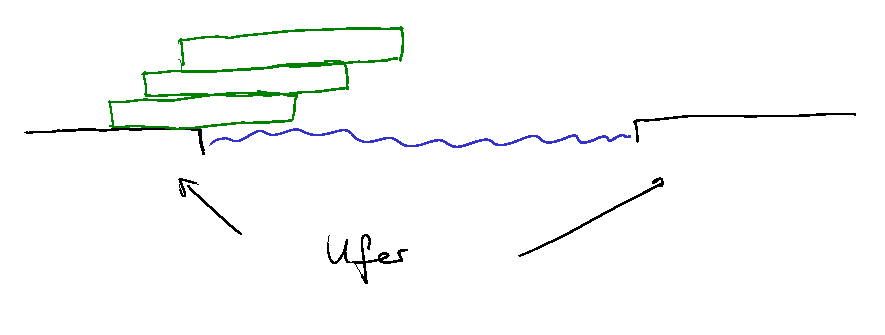
\includegraphics{romeo.pdf}
\caption{Romeos Br\"ucke}\label{fig:romeo} 
\end{figure}
%
\end{aufg}

\bigskip

\begin{lsg}
\end{lsg}


\bigskip


\begin{aufg}[6 Punkte]
Bestimmen Sie folgende Grenzwerte:
\begin{enumerate}[label=$\mathrm{(\roman*)}$, ref=$\mathrm{\roman*}$]
\setlength{\itemsep}{4pt}
\item $ \lim\limits_{x\to \infty} \dfrac{x^{2021}-17x^{10}}{x^{2022}+x+3} $,
\item $ \lim\limits_{x\to 2} \dfrac{x^{2}-3x+2}{x^{2}-x-2} $,
\item $ \lim\limits_{x\to 2} \left(1-\dfrac{2}{x}\right)^{2} \left( \dfrac{x^{7}-4x}{(x-2)^{2}} \right) $.
\end{enumerate}
\end{aufg}

\bigskip

\begin{lsg}\mbox{ }
\begin{enumerate}[label=$\mathrm{(\roman*)}$, ref=$\mathrm{\roman*}$]
\setlength{\itemsep}{4pt}
\item 
\end{enumerate}
\end{lsg}

\bigskip

\begin{aufg}[6 Punkte]
Die Exponentialfunktion $\exp\colon\R\to\R$ ist gegeben durch (siehe Vorlesung)
\[
\exp(x)\coloneqq \sum_{k=0}^{\infty}\frac{x^k}{k!}\,. 
\]
\begin{enumerate}[label=$\mathrm{(\roman*)}$, ref=$\mathrm{\roman*}$]
\item Zeigen Sie, dass $\exp(x)\cdot \exp(y)=\exp(x+y)$ \emph{(Hinweis: Cauchy-Produkt)}.
\item Zeigen Sie, dass die Exponentialfunktion auf ganz $\R$ stetig ist, d.h., f\"ur jedes~$x_0\in\R$ ist der Grenzwert von~$\exp$ in~$x_0$ gerade $\exp(x_0)$.
\end{enumerate}
\end{aufg}
 
\bigskip

\begin{lsg}\mbox{ }
\begin{enumerate}[label=$\mathrm{(\roman*)}$, ref=$\mathrm{\roman*}$]
\item 
\end{enumerate}
\end{lsg}

\bigskip


\begin{aufg}[6 Punkte]
Die \textit{Riemannsche Zeta-Funktion} wird definiert durch die Reihe 
\[
\zeta(s) = \sum_{k=1}^{\infty} \frac{1}{k^{s}}
\]
f\"ur alle $s\in \R$, $s>1$. Zeigen Sie, dass $\zeta(n) < 2$ f\"ur alle nat\"urlichen Zahlen $n\geq 2$. 

\noindent
\emph{Hinweis:} Betrachten Sie zuerst
\[
\sum_{n=2}^{\infty} \sum_{k=2}^{\infty} \frac{1}{k^{n}}\,.
\]
\end{aufg}


\bigskip

\begin{lsg} 
\end{lsg}
 
\bigskip

\begin{aufg}[2 Punkte; Sonderaufgabe]
Wenn Sie Aufgabe~8.5 abgegeben haben (womit Sie sich 2 Punkte verdient haben), erhalten Sie von ihrer \"Ubungsleiterin oder Ihrem \"Ubungsleiter die Abgabe einer anderen Gruppe. Korrigieren Sie diese Abgabe und bepunkten Sie sie. Sie haben 6 Punkte zur Verf\"ugung. (Die andere Gruppe erh\"alt nicht die Punkte, die Sie vergeben, sondern die 2 Punkte f\"ur das Abgeben.) Achten Sie beim Korrigieren insbesondere auf Folgendes: 
\begin{itemize}
 \item Alle Stellen, die falsch sind, anmerken und erkl\"aren, was falsch ist.
 \item Alle Stellen, die unverst\"andlich sind, anmerken und erkl\"aren, was unverst\"andlich ist.
\end{itemize}
Kurzum, Sie machen die Korrektur so, wie Sie erwarten, dass Ihre Abgaben korrigiert werden. Ihr Korrekturergebnis soll so sein, dass Sie hinterher erkl\"aren k\"onnen, was falsch und was richtig an der Abgabe ist. Sie geben die Korrektur dann mit Ihrer Abgabe von Blatt~9 am 21.12. in den \"Ubungsgruppen ab.
\end{aufg}


\newpage
\section{Blatt}

\begin{aufg}[6 Punkte]
Zeigen Sie:
\begin{enumerate}[label=$\mathrm{(\roman*)}$, ref=$\mathrm{\roman*}$]
\item Die Reihe
\[
 \sum_{n=1}^\infty \ln\left( 1 + \frac{1}{n^p} \right)
\]
divergiert f\"ur $p=1$, aber konvergiert f\"ur $p=2$.
\item Die Funktion 
\[
 f\colon (0,\infty)\to\R\,,\quad x\mapsto x + e^{-x} - C
\]
besitzt f\"ur jedes $C>1$ eine Nullstelle. Was passiert f\"ur $C=1$ und was f\"ur $C<1$?
\item Jedes reelle Polynom vom Grad~$3$ besitzt mindestens eine reelle Nullstelle.
\end{enumerate}
\end{aufg}


\bigskip

\begin{lsg}\mbox{ }
\begin{enumerate}[label=$\mathrm{(\roman*)}$, ref=$\mathrm{\roman*}$]
\item 
\end{enumerate}
\end{lsg}


\bigskip


\begin{aufg}[6 Punkte]
Sei die Funktion $f\colon\R\rightarrow\R$ definiert durch 
\[
f(x)\coloneqq \left| \left\lfloor x+\frac{1}{2} \right\rfloor -x \right|\,.
\]
Zeichnen Sie den Graphen der Funktion $f$ in ein geeignetes Koordinatensystem und zeigen Sie:
\begin{enumerate}[label=$\mathrm{(\roman*)}$, ref=$\mathrm{\roman*}$]
    \item F\"ur alle $x\in\R$ gilt $0\le f(x) \le \frac{1}{2}$.
    \item F\"ur alle $x\in \R$ und $n\in\Z$ gilt $f(x+n)=f(x)$.
    \item Die Funktion $f$ ist stetig.
\end{enumerate}
\end{aufg}

\bigskip

\begin{lsg}
\end{lsg}


\bigskip

\begin{aufg}[6 Punkte]
Berechnen Sie den punktweisen Grenzwert der folgenden Funktionenfolgen~$(f_n)_{n\in\N}$ und entscheiden Sie, ob die Konvergenz gleichm\"a{\ss}ig ist:
\begin{enumerate}[label=$\mathrm{(\roman*)}$, ref=$\mathrm{\roman*}$]
\item $f_n(x) = \begin{cases} 0 & x \leq n \\ x-n & x > n \end{cases}$ auf
${}]-\infty, 196560]$ und auf $\R$.
\item $f_n(x) = \frac{x}{1+(nx)^2}$ auf $\R$.
\end{enumerate}
\end{aufg}
 
\bigskip

\begin{lsg}\mbox{ }
\begin{enumerate}[label=$\mathrm{(\roman*)}$, ref=$\mathrm{\roman*}$]
\item 
\end{enumerate}
\end{lsg}

\bigskip

\begin{aufg}[6 Punkte]\mbox{ }
\begin{enumerate}[label=$\mathrm{(\roman*)}$, ref=$\mathrm{\roman*}$]
\item Beweisen Sie folgende Aussage: Sei $(a_n)_{n\in\N}$ eine positive, monoton fallende Nullfolge. Dann konvergiert die Reihe 
\[
\sum_{n=1}^{\infty}a_n
\]
genau dann, wenn die \emph{verdichtete} Reihe 
\[
\sum_{k=0}^{\infty}2^k a_{2^k}
\]
konvergiert. 
\item Nutzen Sie diese Aussage, um das Konvergenzverhalten der Reihe 
\[
\sum_{k=1}^{\infty}\frac{1}{n^a}
\]
f\"ur $a>0$ zu untersuchen. 
\end{enumerate}
\end{aufg}

\bigskip

\begin{lsg}\mbox{ }
\begin{enumerate}[label=$\mathrm{(\roman*)}$, ref=$\mathrm{\roman*}$]
\item 
\end{enumerate}
\end{lsg}

\bigskip


\begin{aufg}[8 Punkte; Bonusaufgabe]\mbox{ }
\begin{enumerate}[label=$\mathrm{(\roman*)}$, ref=$\mathrm{\roman*}$]
\item (Fr\"uhpusher-Bonus) Laden Sie bis zum 18.01.2022, 12:00 Uhr, im git eine L\"osung zu einer Aufgabe der Bl\"atter~$1$-$9$ hoch, die bislang noch keine L\"osung hat. Damit erf\"ullen Sie auch zugleich einen Teil Ihrer Studienleistung. Wenn Sie das schon gemacht haben, erhalten Sie diese~$4$ Bonuspunkte automatisch.
%
\item F\"ur genau welche $x\in\R$ konvergiert die Reihe
\[ 
\sum_{n=1}^\infty\left(x+\frac{1}{n}\right)^n\,?
\]
\end{enumerate}
\end{aufg}


\bigskip

\begin{lsg}
\end{lsg}


\newpage
\section{blatt}

\begin{aufg}[6 Punkte]
Gegeben sei die Funktion $f\colon [0,1]\to\R$ mit 
\[
 f(x) \coloneqq 
 \begin{cases}
  \frac1q & \text{f\"ur~$x>0$ mit $x=\frac{p}{q}$ mit $p,q\in\N$ 
teilerfremd},
  \\
  0 & \text{f\"ur $x$ irrational},
  \\
  1 & \text{f\"ur $x=0$}.
 \end{cases}
\]
Untersuchen Sie, in welchen Punkten $f$ stetig und in welchen Punkten unstetig 
ist.
\end{aufg}

\bigskip


\begin{lsg}
\end{lsg}


\bigskip


\begin{aufg}[6 Punkte] \mbox{ }
\begin{enumerate}[label=$\mathrm{(\roman*)}$, ref=$\mathrm{\roman*}$]
\item Die \textbf{Sinusfunktion/-reihe} ist definiert durch 
\[
 \sin(x) \coloneqq \sum_{k=0}^\infty (-1)^k \frac{x^{2k+1}}{(2k+1)!}\,.
\]
Die \textbf{Kosinusfunktion/-reihe} ist definiert durch 
\[
 \cos(x) \coloneqq \sum_{k=0}^\infty (-1)^k \frac{x^{2k}}{(2k)!}\,.
\]
Zeigen Sie, dass diese beiden Reihen auf jeder beschr\"ankten Teilmenge 
von~$\R$ gleichm\"a{\ss}ig konvergieren und dass beide Funktionen auf ganz~$\R$ 
stetig sind.
%
\item Zeigen Sie, dass die Potenzreihe
\[
 \sum_{k=0}^\infty x^k
\]
auf $(-1,1)$ nicht gleichm\"a{\ss}ig konvergiert, aber auf jeder beschr\"ankten 
Teilmenge von~$(-1,1)$.
\end{enumerate}
\end{aufg}

\bigskip


\begin{lsg}\mbox{ }
\begin{enumerate}[label=$\mathrm{(\roman*)}$, ref=$\mathrm{\roman*}$]
\item 
\end{enumerate}
\end{lsg}


\bigskip


\begin{aufg}[6 Punkte]
Berechnen Sie den Konvergenzradius der folgenden Potenzreihen
\begin{enumerate}[label=$\mathrm{(\roman*)}$, ref=$\mathrm{\roman*}$]
\item $\sum_{k=0}^\infty \frac{k+1}{3^k}x^k$
\item $\sum_{k=10}^\infty \frac{(x-12)^{2k}}{1+\frac{1}{k}}$
\item $\sum_{k=2}^\infty k\cdot (x+3)^k$
\item $\sum_{k=0}^\infty \binom{3k}{k} x^k$.
\end{enumerate}
\end{aufg}
 
\bigskip


\begin{lsg}\mbox{ }
\begin{enumerate}[label=$\mathrm{(\roman*)}$, ref=$\mathrm{\roman*}$]
\item 
\end{enumerate}
\end{lsg}


\bigskip


\begin{aufg}[6 Punkte]
Zeigen Sie, dass folgende (Anf\"ange von) Potenzreihenentwicklungen gelten (auf 
den Definitionsbereich achten!):
\begin{enumerate}[label=$\mathrm{(\roman*)}$, ref=$\mathrm{\roman*}$]
\item $\sin^3 x = x^3 -\frac12x^5 + \frac{13}{120}x^7 + \ldots$ f\"ur alle 
$x\in\R$,
\item $e^{-x}\sin x = x - x^2 + \frac13x^3 - \ldots$ f\"ur alle $x\in\R$,
\item $\frac{e^x \sin x}{\cos^2 x} = x + x^2 + \frac43 x^3 + x^4 + \ldots$ 
f\"ur hinreichend kleines~$|x|$.
\end{enumerate}
Hierbei ist $\sin^3 x \coloneqq (\sin x)^3$, analog f\"ur $\cos^2 x$.
\end{aufg}


\bigskip


\begin{lsg}\mbox{ }
\begin{enumerate}[label=$\mathrm{(\roman*)}$, ref=$\mathrm{\roman*}$]
\item
\end{enumerate}
\end{lsg}

\bigskip


\begin{aufg}[4 Punkte; Bonusaufgabe]
Untersuchen Sie die Funktionenfolge $(f_n)_n$ mit 
\[
 f_n(x) \coloneqq \sqrt[x]{(x^2+2)^2}
\]
hinsichtlich punktweiser und gleichm\"a{\ss}iger Konvergenz auf~$\R$.
\end{aufg}


\bigskip

\begin{lsg}
\end{lsg}

 


\vspace*{.5cm}


\textbf{\LARGE Wichtig:} Dieses ist das letzte \"Ubungsblatt, das in Analysis~1 
bewertet wird. Das n\"achste \"Ubungsblatt ist ein Ferienblatt, das zu Beginn 
von Analysis~2 besprochen wird (zumindest f\"ur Nicht-Lehramt). \"Uberpr\"ufen 
Sie nun folgendes f\"ur die Studienleistung:
\begin{itemize}
\item Haben Sie $50\%$ aller \"Ubungspunkte erreicht? (Die \"Ubungsleiter*innen 
k\"onnen Ihnen dabei helfen.)
\item Haben Sie zwei Aufgaben vorgerechnet?
\item Haben Sie die L\"osung einer Aufgabe ins git gepusht?
\end{itemize}
Wenn Ihnen noch etwas fehlt, versuchen Sie es noch zu schaffen. 

F\"ur die Nicht-Lehr\"amtler: Abgabe der Plenumsmappen bis 05.02.2022 (in 
Ausnahmef\"allen Verl\"angerung bis 11.02.2022). Sie k\"onnen die Plenumsmappen 
mir per Email senden oder auch ins Postfach legen (Fach~90 im MZH, Ebene~1, 
zwischen Senatssaal und Fahrst\"uhlen).

\setlength{\parindent}{0pt}

\end{document}

\newpage
\input{Blatt12}
\newpage
\input{Blatt13}
\end{comment}

\setlength{\parindent}{0pt}

\end{document}
